\chapter{ОНОЛЫН СУДАЛГАА}
\begin{sloppy}

%=============================================================================
\section{AR технологийн онолын үндэс ба мобайл хэрэгжүүлэлт}
%=============================================================================

Өргөтгөсөн бодит байдал (Augmented Reality, AR) нь бодит орчныг виртуал объект, тайлбар, дүрслэл, аудио, интерактив элементээр баяжуулж, хэрэглэгчид бодит ба дижитал орчныг нэгэн зэрэг мэдрэх боломж олгодог технологи юм \cite{Azuma1997,Milgram1994}. AR-ийн үндсэн шинж нь бодит орчныг орлуулах бус, түүнд утга нэмж өгөхөд оршдог. Энэ нь аялал жуулчлалын хэрэглээнд онцгой ач холбогдолтой. Жуулчин бодит газар дээрээ байж, тухайн байршилтай холбоотой түүх, домог, соёлын өгүүлэмжийг нэмэлт хэлбэрээр хүлээн авах тул AR нь destination replacement бус destination enrichment буюу байршлын үнэ цэнийг өргөтгөх хэрэгсэл болдог \cite{Kounavis2012TourismAR}.

AR системийг marker-based, markerless, location-based, projection-based болон superimposition-based хэлбэрт ангилж болдог \cite{Billinghurst2015ARSurvey,Brito2017MarkerVsMarkerless}. Энэхүү дипломын ажлын судалгааны объект нь markerless ба location-based AR-ийн хосолсон загвар юм. Өөрөөр хэлбэл контент нээх шийдвэрийг GPS ба LBS түвшинд гаргаж, виртуал объектыг бодит орчинд байрлуулахдаа plane detection, tracking, anchor зэрэг AR-ийн локал механизм ашиглаж байна. Энэ хосолсон хэлбэр нь зөвхөн GPS эсвэл зөвхөн markerless хандлагаас илүү практик шийдэлд тооцогдоно.

\subsection{Мобайл AR-ийн техникийн тулгуур}

Мобайл AR нь камерын дүрс дээр 3D загвар давхарлах энгийн аргачлал бус, харин мэдрэгчийн нийлмэл экосистемд тулгуурласан бодит цагийн тооцооллын систем юм. Гол мэдрэгчүүдэд RGB камер, акселерометр, гироскоп, magnetometer, GPS болон зарим төхөөрөмжийн LiDAR багтана \cite{Haneefa2024,Syed2022ARTracking}. Камер нь дүрсийн онцлог цэгүүдийг илрүүлж tracking хийхэд, IMU нь хурдан хөдөлгөөний өөрчлөлт барихад, GPS нь үнэмлэхүй байршлын бүдүүн түвшний мэдээлэл өгөхөд ашиглагддаг. Нэг мэдрэгч дангаараа хангалтгүй тул sensor fusion зайлшгүй шаардлагатай.

Мобайл AR-д дэлхийн координат, төхөөрөмжийн координат, AR world coordinate гэсэн дор хаяж гурван координатын тогтолцоо зэрэг оролцдог. Географийн координатыг контент идэвхжүүлэх логикт ашиглах боломжтой боловч виртуал авдрыг дэлгэц дээр тогтвортой дүрслэхэд локал AR world coordinate шаардлагатай. Иймээс хэрэглэгч тухайн цэгт хүрсэн эсэхийг
\[
d(\mathbf{p}_{user}, \mathbf{p}_{spot}) \le r
\]
нөхцлөөр шалгаж, нөхцөл биелсний дараа авдрыг локал хавтгай дээр anchor ашиглан байрлуулах нь архитектурын зөв салгалт болно.

\subsection{AR pipeline, SLAM ба visual-inertial odometry}

Мобайл AR системийн ажиллагааг camera and IMU input $\rightarrow$ feature tracking $\rightarrow$ plane detection $\rightarrow$ pose estimation $\rightarrow$ anchor placement $\rightarrow$ rendering гэсэн шаталсан pipeline-ээр тайлбарлах нь оновчтой \cite{Arena2022AROverview,Haneefa2024}. Энэ дамжуулах хоолойн цөмд markerless tracking оршдог бөгөөд түүнийг SLAM болон visual-inertial odometry (VIO) дэмждэг. SLAM нь орчны газрын зураг үүсгэхийн зэрэгцээ төхөөрөмжийн pose-ийг үнэлдэг бол VIO нь камерын харааны мэдээлэл ба IMU өгөгдлийг нэгтгэн хөдөлгөөнийг илүү тогтвортой тооцоолдог \cite{Syed2022ARTracking}.

Энэ механизмыг дараах магадлалт үнэлгээгээр илэрхийлж болно.
\[
P(x_{1:t}, m \mid z_{1:t}, u_{1:t}),
\]
энд $x_t$ нь төхөөрөмжийн pose, $m$ нь map, $z_t$ нь ажиглалт, $u_t$ нь IMU-ийн хөдөлгөөний мэдээлэл юм. Практикт AR Foundation, ARKit, ARCore зэрэг платформууд энэхүү тооцооллыг дотоод түвшинд гүйцэтгэдэг боловч системийн хязгаарлалтыг ойлгохын тулд дээрх онолын суурь зайлшгүй шаардлагатай.

\subsection{Sensor fusion ба тогтвортой дүрслэлийн математик үндэс}

Gyroscope богино хугацаанд хөдөлгөөнийг сайн барьдаг боловч drift хуримтлагддаг; accelerometer нь таталцлын чиглэл өгдөг ч шуугианд мэдрэмтгий; GPS нь байршлын үнэмлэхүй мэдээлэл өгдөг ч шинэчлэл удаан, алдаатай байдаг. Иймд complementary filter, Kalman filter, EKF зэрэг аргаар мэдрэгчийн мэдээллийг нэгтгэх шаардлагатай \cite{Syed2022ARTracking,Kaplan2006}. Энгийн complementary filter-ийг дараах байдлаар томьёолж болно.
\[
\theta_t = \alpha(\theta_{t-1} + \omega_t \Delta t) + (1-\alpha)\theta^{acc}_t,
\]
энд $\omega_t$ нь gyro хэмжилт, $\theta^{acc}_t$ нь accelerometer-ийн үнэлгээ, $\alpha$ нь жингийн коэффициент юм. Энэхүү томьёо нь визуал стабилизаци ба орон зайн байршуулалтын ард олон мэдрэгчийн тэнцвэржүүлэлт явагддагийг харуулна.

Текстэн зураглалын тайлбар: энэхүү судалгаанд GPS нь байршилд хүрсэн эсэхийг шалгах макро механизм, AR tracking нь виртуал объектыг тогтвортой дүрслэх микро механизм гэж тусгаарлагдана. Ингэснээр GPS-ийн 5--15 метрийн хэлбэлзлийг дэлгэц дээрх объектын байрлалд шууд дамжуулахгүй.

Энэ хэсгийн онол нь дипломын ажлын дараагийн бүлэгт сонгох ``радиуст суурилсан идэвхжилт + динамик AR байршуулалт'' шийдлийг үндэслэж байна. Өөрөөр хэлбэл Unity төвтэй хэрэгжилтийн үед байршлын триггер ба дүрслэлийн триггерийг салгах шаардлагыг энэ онол тайлбарлаж өгнө.

%=============================================================================
\section{Байршилд суурилсан үйлчилгээ ба контекст-мэдрэмтгий систем}
%=============================================================================

Байршилд суурилсан үйлчилгээ (LBS) нь хэрэглэгчийн физик байршлыг ашиглан контент, үйлчилгээ, зөвлөмж, мэдэгдэл хүргэдэг мэдээллийн систем юм \cite{Virrantaus2001}. Аялал жуулчлалын орчинд LBS нь газрын зураг үзүүлэхээс илүү өргөн үүрэгтэй. Энэ нь хэрэглэгч ``хаана байна'' гэсэн асуултыг ``энэ байршилд ямар утга, контент, үйл ажиллагаа нээгдэх вэ'' гэсэн утгатай холбодог. Иймээс LBS нь AR аялал жуулчлалын системд навигацийн туслах бус, тоглоомын логикийн үндсэн оролцогч болж хувирна.

\subsection{Контекст-мэдрэмтгий тооцоолол}

Контекст нь зөвхөн байршлаар хязгаарлагдахгүй. Контекст-мэдрэмтгий тооцооллын судалгаагаар хэрэглэгчийн үйл ажиллагаанд хамааралтай аливаа мэдээллийг контекст гэж үздэг \cite{Schilit1994,Dey2001}. Үүнд байршил, цаг хугацаа, төхөөрөмжийн төлөв, сүлжээний боломж, орчны гэрэлтүүлэг, өмнөх үйлдэл, хэрэглэгчийн зорилго зэрэг орно. Аялал жуулчлалын системд энэ ойлголт маш чухал. Учир нь нэг ижил байршил дээр ч өглөө, орой, сүлжээ тасарсан үе, эсвэл тухайн шагналыг өмнө нь авсан эсэхээс шалтгаалан системийн хариу өөр байх ёстой.

Текстэн диаграмын тайлбар: байршлын шинэчлэлт ирэхэд систем эхлээд accuracy шалгалт хийнэ. Дараа нь шүүсэн координатыг аяллын цэгүүдтэй харьцуулж, радиусын нөхцөл биелсэн эсэхийг тооцно. Үүний дараа тухайн хэрэглэгч уг шагналыг өмнө нь авсан эсэх, төхөөрөмж AR session эхлүүлэхэд бэлэн эсэх, сүлжээний орчин тасалдсан эсэхийг шалгаж байж эцсийн trigger үүсгэнэ. Энэ урсгал нь location-aware механизмыг context-aware систем болгон өргөтгөж байгаа хэлбэр юм.

\subsection{Радиуст суурилсан идэвхжилт, шүүлт ба hysteresis}

GPS хэмжилт бодит орчинд савлах шинжтэй тул яг нэг координаттай давхцах хатуу нөхцөл хэрэглэх нь практик хэрэглээнд тохиромжгүй. Иймээс идэвхжилтийг радиустай бүсээр загварчилж, Haversine томьёогоор зай тооцоолох нь оновчтой \cite{Kaplan2006}. Зайг дараах байдлаар тооцож болно.
\[
\Delta d = 2R \arcsin \sqrt{\sin^2\left(\frac{\Delta \phi}{2}\right) + \cos \phi_1 \cos \phi_2 \sin^2\left(\frac{\Delta \lambda}{2}\right)}.
\]
Энд $R$ нь дэлхийн радиус, $\phi$ нь өргөрөг, $\lambda$ нь уртраг байна.

GPS савлалтын нөлөөг багасгахын тулд smoothing ба hysteresis хэрэглэнэ. Жишээлбэл шүүсэн координатыг
\[
\hat{p}_t = \beta p_t + (1-\beta)\hat{p}_{t-1}
\]
гэсэн экспоненциал шүүлтээр тооцож, дараа нь `enter' ба `exit' хоёр босго ашиглан төлөв солигдох давтамжийг бууруулж болно:
\begin{align}
\text{Enter if } & d \le r_{enter}, \\
\text{Exit if } & d > r_{exit}, \qquad r_{exit} > r_{enter}.
\end{align}
Энэ арга нь радиусын хил дээр олон дахин мэдэгдэл үүсэх, AR товч байнга асаж унтрах зэрэг UX-ийн доголдлыг бууруулна.

\subsection{LBS ба AR-ийн хосолсон архитектурын ач холбогдол}

Байршлын систем ба AR session-ийг салангид боловч уялдаатайгаар авч үзэх нь инженерийн чухал шийдвэр юм. LBS нь аль цэг дээр аль контентыг нээх вэ гэдгийг тодорхойлж, AR механизм нь тэр контентыг хэрхэн харагдуулах вэ гэдгийг шийднэ. Хэрэв GPS-ийн хэмжилтийг шууд объектын 3D байрлалд хэрэглэвэл объект газарт шургах, хэт хол харагдах, хэрэглэгч төөрөх эрсдэлтэй. Харин GPS-ийг trigger-д, AR plane placement-ийг орон зайн дүрслэлд ашиглавал системийн тогтвортой байдал нэмэгдэнэ.

Энэ хэсгийн онол нь системийн зохиомжийн бүлэгт байршлын триггер, мэдэгдэл, AR нээх нөхцөл, fallback шийдлүүдийг тайлбарлах үндэс болно. Ялангуяа cached spot data, offline мэдээлэл, already claimed төлөв зэрэг бизнес дүрмүүдийг контекстийн нэг хэсэг болгон авч үзэх боломжийг нээж өгч байна.

%=============================================================================
\section{Тоглоомжуулалт, хэрэглэгчийн оролцоо ба AR UX}
%=============================================================================

Тоглоомжуулалт нь тоглоом биш орчинд тоглоомын дизайн, механик, урамшууллын элемент ашиглан оролцоо, сэдэл, зорилтот үйлдлийг нэмэгдүүлэх аргачлал юм \cite{Deterding2011Gamification,Hamari2014}. Аялал жуулчлалын хувьд тоглоомжуулалт нь газар үзэх үндсэн зорилгыг өөрчилдөггүй, харин түүнийг зорилготой, шатлалтай, шагналтай, дахин ашиглах хүсэл төрүүлэх туршлага болгодог \cite{Xu2017GamificationTourism}. Treasure hunt, collection, achievement, stamp, progress tracking зэрэг механик нь энэ салбарт түгээмэл ашиглагддаг.

Механик--динамик--туршлага (MDA) хандлагаар авч үзвэл ``байршилд хүрэх'', ``авдар нээх'', ``шагнал цуглуулах'' нь механик; ``судлах хүсэл'', ``ахицын мэдрэмж'', ``нээлтийн сонирхол'' нь динамик; ``сэтгэл ханамж'', ``оролцооны гүн'', ``утга олж авах'' нь туршлагын түвшин юм. Иймээс аялал жуулчлалын AR тоглоомын дизайнд зөвхөн шагнал өгөхөөс илүү тухайн шагналын соёлын тайлбар, байршилтай уялдсан өгүүлэмж чухал байр эзэлнэ.

\subsection{Self-Determination Theory ба Flow}

Деки ба Райаны өөрөө тодорхойлох онолын дагуу хүний дотоод сэдэл autonomy, competence, relatedness гэсэн гурван хэрэгцээтэй холбоотой \cite{Deci1985,Ryan2000}. AR аялал жуулчлалын тоглоомд autonomy нь хэрэглэгч аль байршлаас эхлэхээ сонгох боломжоор, competence нь цуглуулга нэмэгдэх ахицын мэдрэмжээр, relatedness нь соёлын утгатай reward ба маршрутын өгүүлэмжээр илэрнэ. Иймд reward нь зөвхөн гадаад урамшуулал бус, Монголын ахуй, түүх, соёлын утгыг дамжуулах дотоод сэдлийн хэрэгсэл болж чадна.

Чиксентмихайгийн Flow онол нь сорилт ба хэрэглэгчийн чадамж тэнцвэртэй үед төвлөрөл, сэтгэл ханамж, цаг хугацааны мэдрэмж алдагдах өндөр оролцооны төлөв үүсдэгийг тайлбарладаг \cite{Csikszentmihalyi1990}. Аялал жуулчлалын нөхцөлд хэт олон дүрэм, төвөгтэй мини тоглоом нь хэрэглэгчийг ядрааж болзошгүй. Харин ``байршилд хүрэх $\rightarrow$ AR нээх $\rightarrow$ авдар олох $\rightarrow$ шагнал авах'' гэсэн богино, ойлгомжтой урсгал нь flow-ийг дэмжих магадлал өндөртэй.

\subsection{User engagement, immersion ба AR UX}

Хэрэглэгчийн оролцоо нь зөвхөн апп дээр өнгөрүүлсэн хугацаагаар хэмжигдэхгүй; анхаарал, сэтгэл хөдлөл, танин мэдэхүйн оролцоо, дахин ашиглах хүсэл, утга олж авах түвшинг хамардаг \cite{OBrien2008,Lehmann2012}. Мобайл AR нь VR шиг бүрэн тусгаарласан immersion үүсгэдэггүй ч бодит орчинд суурилсан presence буюу ``энэ контент яг энд байна'' гэсэн мэдрэмжийг бий болгодог \cite{Bowman2007}. Аялал жуулчлалын хэрэглээнд энэ нь өндөр үнэ цэнтэй, учир нь хэрэглэгч тухайн дурсгалт газар дээр бодитоор зогсож байхдаа контентыг хүлээн авдаг.

AR UX-ийн хувьд spatial clarity, interaction simplicity, visual stability, contextual relevance, safety-aware design гэсэн таван зарчим хамгийн чухал \cite{Yovcheva2014AugmentedTourism}. Тиймээс авдрыг хэрэглэгчийн өмнө ойлгомжтой зайд байрлуулах, нэг товшилтоор харилцах, шагналын тайлбарыг хэт урт биш боловч соёлын утга агуулсан байлгах, алхаж явах үед анхаарал сарниулахгүй интерфэйс хэрэглэх шаардлагатай.

\subsection{Соёлын контентыг тоглоомжуулсан хэлбэрт шилжүүлэх үндэслэл}

Монголын аялал жуулчлалын контентод уяа сойлго, хөөрөг, дээл, ааруул, айраг, түүхэн баатрын домог, байршил тус бүрийн өгүүлэмж зэрэг соёлын элементүүдийг reward хэлбэрээр оруулах нь тоглоомжуулалтыг утгагүй урамшууллын систем болохоос сэргийлнэ. Reward бүр танин мэдэхүйн тайлбар агуулснаар тоглоомын механик ба боловсролын үнэ цэнийг нэгтгэнэ. Энэ нь gamified learning болон tourism interpretation-ийн завсрын хэлбэр гэж үзэж болно \cite{Xu2017GamificationTourism,Jo2025ARGamification}.

Энэ хэсгийн онол нь системийн зохиомжийн бүлэгт collection system, reward panel, collection retrieval, progress visibility, хэрэглэгчийн урсгалын энгийн байдлыг хэрхэн тайлбарлахыг тодорхойлж байна. Өөрөөр хэлбэл UX-ийн шийдвэр бүрийн ард сэтгэлзүй ба оролцооны онолын шалтгаан байгааг энэ хэсэг нотолж өгнө.

%=============================================================================
\section{Системийн архитектур ба алгоритмын загвар}
%=============================================================================

Мобайл AR аялал жуулчлалын системийг дөрвөн үндсэн давхаргатайгаар авч үзэж болно: хэрэглэгчийн интерфэйсийн давхарга, AR боловсруулах давхарга, бизнес логикийн давхарга, өгөгдөл ба үйлчилгээний давхарга. Интерфэйсийн давхарга нь газрын зураг, AR view, reward panel, collection дэлгэцийг хариуцна. AR давхарга нь session, plane detection, anchor, rendering-ийг зохицуулна. Бизнес логик нь байршлын trigger, reward rules, collection state, already claimed төлөвийг удирдана. Өгөгдлийн давхарга нь API, өгөгдлийн сан, аяллын цэгийн мета мэдээлэл, цуглуулгын түүхийг хадгална.

Текстэн зураглалын тайлбар: хэрэглэгч байршлын шинэчлэлт авахад клиент тал TourismSpotManager-аар ойролцоох цэгүүдийг тооцно. Хэрэв триггерийн нөхцөл биелбэл интерфэйс AR нээх боломж идэвхжүүлнэ. AR scene руу шилжихэд ARChestSpawner тохирох хавтгай илрүүлж авдар байрлуулна. Хэрэглэгч авдрыг нээмэгц ARChestInteraction визуал урсгалыг ажиллуулж, backend талд reward claim хүсэлт илгээгдэнэ. Амжилттай бол collection state шинэчлэгдэнэ.

\subsection{AR placement scoring ба fallback логик}

Бодит орчинд хэд хэдэн candidate plane илэрсэн үед объект аль гадаргуу дээр харагдах ёстойг онооны функцээр эрэмбэлж болно. Нийтлэг хэлбэр нь
\[
S_i = w_1 \cdot vis_i + w_2 \cdot stab_i + w_3 \cdot dist_i - w_4 \cdot tilt_i
\]
байж болно. Энд $vis_i$ нь харагдах байдал, $stab_i$ нь tracking-ийн тогтвортой байдал, $dist_i$ нь хэрэглэгчээс тохиромжтой зай, $tilt_i$ нь налуугийн алдагдлыг илэрхийлнэ. Хэрэв хангалттай plane олдохгүй бол fallback chest placement хэрэглэгчийн өмнө тогтоосон зайд объект үүсгэх замаар UX-ийг таслахгүй байлгах боломжтой.

Энэхүү fallback стратеги нь prototype системд онцгой ач холбогдолтой. Учир нь талбайн туршилтын үед гэрэлтүүлэг, шалны текстур, хөдөлгөөн зэргээс хамаарч plane detection тогтворгүй байж болно. AR туршлага бүрэн тасалдахаас илүүтэйгээр controlled fallback хэрэглэснээр хэрэглэгч reward loop-оо дуусгах боломжтой болно.

\subsection{Өгөгдлийн загвар ба бизнес дүрэм}

Системийн өгөгдлийн загвар нь \texttt{User}, \texttt{TourismSpot}, \texttt{Reward}, \texttt{UserReward} гэсэн дөрвөн үндсэн entity дээр тулгуурлана. \texttt{User} нь guest session-ийн үндсэн төлөв, төхөөрөмжийн танигч, display name зэргийг хадгална. \texttt{TourismSpot} нь байршлын нэр, координат, радиус, холбогдох reward-ийн мэдээлэлтэй байна. \texttt{Reward} нь нэр, тайлбар, дүрслэлийн мета мэдээллийг агуулна. \texttt{UserReward} нь аль хэрэглэгч аль байршлаас ямар reward хэзээ авсныг тэмдэглэнэ.

Энэ загварт хамгийн чухал бизнес дүрэм нь нэг хэрэглэгч нэг байршлын шагналыг зөвхөн нэг удаа авах ёстой гэсэн шаардлага юм. Үүнийг өгөгдлийн сангийн түвшинд \texttt{@@unique([userId, tourismSpotId])} хэмжигдэхүүнээр хамгаалснаар клиент талын алдаа, давхар даралт, сүлжээний давтагдсан хүсэлтээс үл хамааран өгөгдлийн бүрэн бүтэн байдал хадгалагдана.

\subsection{API интерфейс ба систем хоорондын гэрээ}

Системийн гол интерфейсүүд нь backend API-гаар тодорхойлогдоно. \texttt{POST /auth/guest-login} endpoint нь guest session үүсгэх буюу сэргээх; \texttt{GET /spots} нь идэвхтэй аяллын цэгүүдийн жагсаалтыг reward мета мэдээллийн хамт татах; \texttt{POST /spots/:id/claim} нь reward claim баталгаажуулах; \texttt{GET /users/:id/rewards} нь хэрэглэгчийн collection retrieval хийх үүрэгтэй. Эдгээр endpoint нь client-side, AR scene, өгөгдлийн сангийн хоорондын гэрээг тогтоож өгнө.

Энэ хэсгийн онол нь хэрэгжилтийн бүлэгт класс, модуль, endpoint, constraint түвшний тайлбарыг эмхтэй ойлгох үндэс болно. Ялангуяа макро ба микро логикийн салгалт, fallback стратеги, unique constraint, collection retrieval зэрэг нь инженерийн шийдвэрийг системийн түвшинд тайлбарлах боломж олгож байна.

%=============================================================================
\section{Case study, ёс зүй ба Монголын нөхцөлд нутагшуулах боломж}
%=============================================================================

\subsection{Харьцуулсан жишээнүүдийн шинжилгээ}

Байршилд суурилсан AR тоглоомын хамгийн өргөн танигдсан жишээ бол Pok\'emon GO юм. Энэхүү систем нь collection mechanic, event-based engagement, газрын зурагт тулгуурласан exploration-ийг амжилттай нэгтгэж, бодит орчин дахь хөдөлгөөнийг нэмэгдүүлсэн \cite{Althoff2016PokemonGO}. Ingress нь байршлыг game board болгон хувиргаж, хотын дурсгалт объектуудыг зангилаа болгон ашигласнаараа онцлог. Харин аялал жуулчлалын зориулалттай gamified passport загварууд, тухайлбал Чианг Май хотын туршлага нь reward collection ба соёлын контентыг маршрутын менежменттэй нэгтгэж болдгийг харуулсан \cite{Thinnukool2025LannaPassport}. Хотын аялал, heritage AR, музейн аппликейшнүүд нь орчныг тайлбарлах, реконструкц хийх, тэмдэг цуглуулах зэрэг механик ашиглан хэрэглэгчийн ойлголтыг гүнзгийрүүлдэг \cite{Yovcheva2014AugmentedTourism,Kounavis2012TourismAR}.

\begin{table}[H]
\centering
\caption{Case study-үүдийн харьцуулсан шинжилгээ}
\label{tab:case-studies}
\begin{tabular}{|p{3cm}|p{3cm}|p{3cm}|p{4cm}|}
\hline
\textbf{Систем} & \textbf{Гол механик} & \textbf{Техникийн тулгуур} & \textbf{Монголын нөхцөлд авах сургамж} \\ \hline
Pok\'emon GO & Collection, event, map exploration & GPS + AR encounter & Collection loop ба дахин ашиглалтыг дэмжих event механик хэрэгтэй \\ \hline
Ingress & Байршлыг тоглоомын талбар болгох & GPS + point-of-interest network & Хотын дурсгалт объектуудыг node хэлбэрээр зохиомжлох боломжтой \\ \hline
Gamified passport & Stamp, маршрут, reward & LBS + lightweight mobile interaction & Маршрут дуусгах, stamp цуглуулах механик жуулчдад ойлгомжтой \\ \hline
Heritage AR apps & Contextual storytelling, reconstruction & AR tracking + multimedia content & Соёлын тайлбар, түүхэн өгүүлэмжийг reward-той холбох шаардлагатай \\ \hline
\end{tabular}
\end{table}

\subsection{Ёс зүй, аюулгүй байдал, хүртээмж}

AR аялал жуулчлалын систем нь хэрэглэгчийг хөдөлгөөнд уриалдаг учраас замын хөдөлгөөн, шат, замбараагүй орон зай, олон хүнтэй бүсэд анхаарал сарниулах эрсдэлтэй \cite{Kounavis2012TourismAR}. Мөн байршлын өгөгдөл нь хувь хүний хөдөлгөөний хэв маягийг илтгэх эмзэг мэдээлэл тул хамгийн бага хэрэгцээтэй түвшинд хадгалах, тасралтгүй мөрдөхөөс зайлсхийх, хэрэглэгчид зөвшөөрлийн тайлбарыг ойлгомжтой өгөх шаардлагатай. Хүртээмжийн үүднээс том товч, тод тайлбар, хөдөлгөөн хязгаарлагдмал хэрэглэгчдэд уян хатан reward loop, AR амжилтгүй үед non-AR fallback тайлбар өгөх нь зүйтэй.

\subsection{Монголын аялал жуулчлалд нутагшуулах боломж}

Монголын нөхцөлд байршил бүрийн reward-ийг соёлын утгатай холбох нь зүйтэй. Жишээлбэл Сүхбаатарын талбайд түүхэн тэмдэгт, Богд хааны ордон орчимд хаадын ёслолын эд зүйл, музейн маршрут дээр тайлбартай collectible card, хөдөөгийн аялалд ахуйн хэрэглээний виртуал үзмэр нээх боломжтой. Ийм reward нь хэрэглэгчийг зөвхөн цуглуулга бүрдүүлэхээс илүү тухайн байршлын утга, түүх, өвөрмөц чанарыг ойлгоход хөтөлнө.

Монголын хотын болон хөдөөгийн нөхцөл ялгаатай тул системийг бүгдэд нь ижил логикоор хэрэглэх боломжгүй. Хотод point-of-interest нягт байрлах тул short-route collection mechanic тохиромжтой бол хөдөө орон нутагт өргөн зай, сул сүлжээ, өөр мэдрэгчийн нөхцөлийг харгалзсан offline-aware дизайн шаардлагатай. Иймээс prototype-ийн архитектур өргөтгөх боломжтой, context-aware, fallback-тэй байх нь зайлшгүй юм.

Энэ хэсгийн шинжилгээ нь энэхүү дипломын ажлын практик чиг баримжааг тодорхойлж байна. Нэг талаас дэлхийн амжилттай жишээнээс collection, маршрутын шатлал, event loop, contextual storytelling-г авна; нөгөө талаас Монголын нөхцөлд crowd management, сүлжээний ялгаа, соёлын агуулгын үнэн зөв байдал, хүртээмжийн асуудлыг заавал тусгана.

\end{sloppy}

%=============================================================================
% НЭМЭЛТ ОНОЛЫН ТОЙМ I: ТОГЛООМЖУУЛАЛТ БА СУРАЛЦАХУЙ
%=============================================================================

\chapter{game-based engagement}
\begin{sloppy}
Геймификаци нь тоглоомын дизайны элементүүдийг тоглоом биш орчинд ашиглахыг хэлдэг бол тоглоомд суурилсан суралцахуй нь өөрөө тоглоомын бүтэц, дүрэм, хийсвэр зөрчил, сорилт, хариу үйлдэл, буцах холбоотой орчныг суралцах зорилгод зориулан зохион бүтээдэг. Иймээс ``оноо нэмэх'' нь дангаараа game-based learning биш; харин сургалтын үйл ажиллагааг тоглоомын логикоор дахин загварчлах үед л game-based learning болно. ``Game-based engagement'' гэх нэр томьёо нь академик талбарт нэг мөр канон тодорхойлолтгүй боловч тоглоомын цикл, сорилт, буцах холбоо, нийгмийн харилцан үйлчлэлийг ашиглан оролцоог тогтвортой өсгөх дизайн-орон зайг илэрхийлдэг гэж ойлгож болно.

Эмпирик судалгааны том зураг нь ``геймификаци үр дүнтэй байж чадна, гэхдээ автоматаар биш'' гэсэн дүгнэлт рүү хүрдэг. Ерөнхий тоймууд ба мета-анализууд геймификаци нь сурлагын танин мэдэхүйн, сэдэлжлийн, зан үйлийн үзүүлэлтүүдэд жижиг боловч эерэг нөлөө өгч болохыг харуулсан; харин нөлөө нь контекст, хэрэглэгчийн төрөл, механикийн хослол, нийгмийн горим, game fiction байгаа эсэх, хэмжилтийн чанараас ихээхэн хамаардаг. Ялангуяа өрсөлдөөнийг хамтын ажиллагаатай хослуулах, тодорхой зорилго, ойрын буцах холбоо, чадвар--сорилтын тэнцвэрийг хангах үед үр нөлөө өсдөг.

Гэхдээ ``оноо, badge, leaderboard = мотиваци'' гэсэн шулуун шугаман ойлголт буруу. Зарим туршилтад points, levels, leaderboards нь гүйцэтгэлийн хэмжээг өсгөсөн ч intrinsic motivation-ийг өсгөөгүй; урт хугацааны анги-танхимын судалгаанд буруу хэрэглэсэн badges + leaderboards нь сэтгэл ханамж, intrinsic motivation, empowerment-ийг бууруулсан тохиолдол ч бий. Тиймээс механик бүр өөр өөр сэтгэлзүйн сувагтай: зарим нь competence, зарим нь relatedness, зарим нь progress visibility, зарим нь novelty ба uncertainty-ээр ажилладаг. Геймификацийн чанар нь механикийн тоонд биш, хэрэгцээ--зан үйл--үр дүнгийн логик нийцэлд оршино.

Энэ тайлангийн гол дүгнэлт дараах таван зарчимд төвлөрнө. Нэгд, гадаад шагнал бус утга учиртай үйл ажиллагааг үндсэн хөдөлгөгч болгох. Хоёрт, autonomy, competence, relatedness-ийг дэмжих. Гуравт, сорилт--чадварын тэнцвэр, тодорхой зорилго, ойрын буцах холбоогоор flow ба immersion-ийг дэмжих. Дөрөвт, engagement-ийг зөвхөн retention-оор бус сэтгэлзүйн болон суралцахуйн үзүүлэлтүүдтэй хослуулж хэмжих. Тавд, өрсөлдөөн, санамсаргүй шагнал, нийгмийн харьцуулалтын ёс зүйн эрсдэлийг урьдчилан удирдах.

%----------------------------------------------------------------------
\section{Үндсэн ойлголт ба түүхэн хөгжил}
%----------------------------------------------------------------------

Геймификацийн орчин үеийн академик тодорхойлолтыг Sebastian Deterding болон хамтран зохиогчид 2011 онд ``game design elements''-ийг ``non-game contexts''-д хэрэглэх гэж томьёолсон. Энэ нь serious games, playful design, alternate reality games зэрэг ойролцоо ойлголтуудаас ялгаатай: тэр бүхэнд тоглоомын бүхэл бүтэн систем чухал байдаг бол gamification-д ихэнхдээ тоглоомын хэсэгчилсэн элементүүдийг үйлчилгээ, сургалт, апп, байгууллагын процесс руу шингээдэг.

Тоглоомд суурилсан суралцахуйг Plass, Homer, Kinzer нар геймификациас ялгаж, тоглоомын дүрэм, хийсвэр зөрчил, сорилт, хариу үйлдэл, буцах холбоогоор суралцах туршлагыг бүхэлд нь зохион байгуулдаг орчин гэж тайлбарласан. Тэдний загварт challenge--response--feedback гэсэн цикл нь тоглоомын сургалтын үндсэн unit бөгөөд game design features нь энэ циклийг ``playful learning'' болгон хувиргадаг. Өөрөөр хэлбэл gamification нь existing task дээр game layer нэмэх хандлагатай бол game-based learning нь task-ийг тоглоомын логикоор дахин зохион бүтээдэг.

``Game-based engagement'' гэдэг нэр томьёо нь нэг мөр стандартчилсан, бүх нийтээр хүлээн зөвшөөрөгдсөн тодорхойлолтгүй. Гэсэн ч хэрэглэгчийн оролцоог тоглоомын бүтцээр удирдах оролдлогуудыг тайлбарлахад уг нэр томьёо аналитик хувьд хэрэгтэй. Ke, Xie, Xie нарын тайлбарласнаар game-based learning engagement нь optimal challenge-оор өдөөгдсөн affective engagement-ээс playfulness-д суурилсан cognitive engagement рүү, цаашлаад агуулгад чиглэсэн engagement рүү ахидаг, үргэлжилсэн интеграцлагдсан үйл явц юм. Энэ санаа нь хэрэглэгчийн оролцоо, суралцах оролцооны орчин үеийн онолуудтай нийцдэг.

Түүхэн хувьд энэ салбар нь behaviorist reinforcement, self-efficacy, goal-setting, expectancy-value, flow, immersion, user engagement, serious games, gamification research гэсэн хэд хэдэн урсгал нийлж хөгжсөн огтлолцол юм. B.F.~Skinner-ийн reinforcement schedules, self-efficacy-ийн чиглэл, Mihaly Csikszentmihalyi-ийн flow, олон талт student/user engagement, immersion-ийн шатлал, улмаар геймификацийн тодорхойлолт, мета-анализууд бүгд нийлж өнөөгийн дизайн ба хэмжилтийн хэл формыг бүрдүүлсэн.

\begin{figure}[htbp]
    \centering
    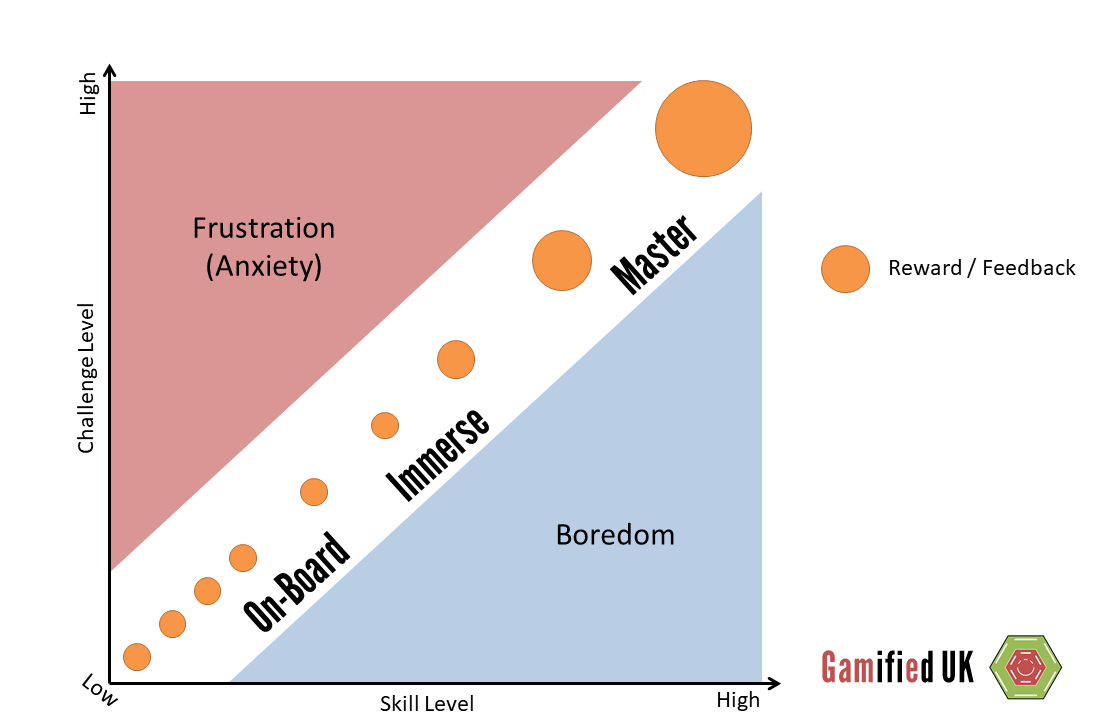
\includegraphics[width=0.8\textwidth]{figures/Slide3.png}
    \caption{Онолын хөгжлийн цаглал}
    \label{fig:theory-timeline}
\end{figure}

Энэ цаглалын логик нь reinforcement-аас motivation, тэндээс experience, дараа нь design framework, эцэст нь evidence synthesis рүү шилжсэн хөгжлийг харуулж байна. Skinner-ийн schedules of reinforcement, Bandura-гийн self-efficacy, flow, MDA, immersion, gamification definition, empirical review, gamified learning theory, meta-analysis зэрэг нь өнөөгийн бүтээгдэхүүн, сургалт, onboarding, loyalty, habit design-д ашиглагдах концепцийн backbone болсон.

Геймификаци, game-based learning, engagement, immersion-ийг тайлбарлахад дан ганц нэг онол хангалтгүй. Сайн дизайн нь behaviorist reinforcement, motivational design, self-determination, goal-setting, expectancy-value, flow, immersion, user engagement, game design framework-уудыг давхар уншиж байж оновчтой болдог. Ялангуяа суралцах болон ажил-гүйцэтгэлийн орчинд ``ямар механик хэрэглэх вэ?'' гэсэн асуултаас илүү ``ямар сэтгэлзүйн хэрэгцээ, ямар зан үйлийг, ямар нөхцөлд өдөөх вэ?'' гэдэг асуулт үр ашигтай.

%----------------------------------------------------------------------
\section{Онол, загваруудын харьцуулсан хүснэгт}
%----------------------------------------------------------------------

\begin{table}[H]
\centering
\caption{Онол болон загваруудын харьцуулалт}
\label{tab:theory-comparison}
\small
\begin{tabular}{|p{2.5cm}|p{3cm}|p{3cm}|p{2.5cm}|p{2cm}|}
\hline
\textbf{Теори / загвар} & \textbf{Гол санаа} & \textbf{Дизайнд өгөх заавар} & \textbf{Давуу тал} & \textbf{Хязгаарлалт} \\ \hline
Өөрөө тодорхойлох онол & Сайн сэдэл ба сайн сайхан байдал нь autonomy, competence, relatedness гэсэн гурван суурь хэрэгцээнээс хамаарна & Сонголт өгөх, mastery feedback өгөх, нийгмийн дэмжлэг бий болгох & Intrinsic ба internalized motivation-ийг тайлбарлахад хүчтэй & Badge/point-ийг controlling болгож хэрэгжүүлбэл сөрөг \\ \hline
Goal-setting theory & Тодорхой, сорилттой зорилго гүйцэтгэлийг чиглүүлж, хүчин чармайлтыг өсгөнө & Ил тод mission, milestone, near-term goal, progress bar ашиглах & Challenge design ба quest architecture-д шууд хэрэглээтэй & Хэт хэцүү goal нь anxiety, disengagement үүсгэж болно \\ \hline
Expectancy-value theory & Хүн амжилт гаргана гэж итгэх ба тухайн даалгаврыг үнэ цэнтэй гэж үзэх үед choice, persistence өснө & Onboarding-оор амжилтын боломжийг ойлгомжтой болгох; relevance-ийг харуулах & Participation ба dropout-ыг сайн тайлбарладаг & Experience design-ийн микро түвшинг төдийлөн задлахгүй \\ \hline
ARCS motivational design & Attention, Relevance, Confidence, Satisfaction гэсэн дөрвөн блокт хувааж motivational design хийдэг & Surprise, meaningful context, scaffolded difficulty, satisfying closure өгөх & Instructional design-т практик хэрэглэхэд хялбар & Хэрэглэгчийн урт хугацааны identity ба social dynamics-ийг бага тайлбарладаг \\ \hline
Flow theory & High challenge + adequate skill, clear goals, feedback, control үед deep involvement үүснэ & Adaptive difficulty, immediate feedback, clear win state, interruption-гүй UX & Immersion ба high-quality engagement-ийг тайлбарлахад төв & Бүх engagement flow биш; low-skill early users-ийг тайлбарлахад хэцүү \\ \hline
Immersion model & Immersion нь engagement $\to$ engrossment $\to$ total immersion гэсэн шатлалтай & Friction-less controls, audiovisual coherence, narrative / attention continuity чухал & UX barriers-ийг оношлоход хэрэгтэй & Субъектив; контекстоос хамааран тодорхойлолт хэлбэлздэг \\ \hline
User engagement framework & Engagement нь aesthetic appeal, focused attention, usability, novelty, endurability зэрэг олон хэмжээсээс бүрдэнэ & Гадаад урамшууллаас гадна usability ба aesthetics-ийг зэрэг сайжруулах & Product analytics ба survey-г холбох боломжтой & Time-on-task гэх мэт single metric хангалтгүй \\ \hline
Gamified Learning Theory & Game attributes нь learning-related behavior / attitude-д нөлөөлж, түүгээрээ суралцах үр дүнд mediating / moderating байдлаар үйлчилнэ & ``Game element $\to$ behavior $\to$ learning outcome'' гэсэн causal chain-аар design хийх & Gamification ба serious games-ийг нэг хүрээнд холбодог & Шууд learning gain-ийг механикаас хэт хамаатуулж тайлбарлах эрсдэлтэй \\ \hline
MDA framework & Mechanics $\to$ dynamics $\to$ aesthetics гэсэн гурван түвшний уялдаа & Component биш, emergent experience-ийг загварчлах & System-level design thinking-д маш хэрэгтэй & Learning / organizational outcomes-ийг дангаараа тайлбарлахгүй \\ \hline
\end{tabular}
\end{table}

Эндээс хамгийн чухал аналитик холбоос нь дараах байдалтай. SDT нь ``яагаад'' гэдгийг, Flow / Immersion нь ``яаж мэдрэгдэж байгааг'', UES нь ``яаж хэмжихийг'', MDA нь ``яаж зохиохыг'', Gamified Learning Theory нь ``ямар замаар үр дүнд хүрэхийг'' тайлбарладаг. Иймээс сайн систем эдгээрийг өрсөлдүүлэх бус давхар уншдаг.

%----------------------------------------------------------------------
\section*{Механизм, дизайн паттерн, оноо--шагнал--түвшин--амжилт--сорилтын архитектур}
%----------------------------------------------------------------------

Платформын түвшинд mechanics, dynamics, aesthetics гэдэг ялгаа чухал. ``Оноо'', ``badge'', ``level'', ``challenge'', ``leaderboard'', ``streak'' нь mechanics; тэдгээрээс төрөх progression, competition, social comparison, curiosity, mastery, commitment нь dynamics; харин achievement, tension, delight, belonging, flow, pressure зэрэг нь хэрэглэгчийн experience юм. Хэрэв дизайнер mechanics түвшинд л гацвал ``шинж тэмдэг'' нэмнэ; харин dynamics ба need satisfaction түвшинг хамтад нь харвал системийн quality сайжирна.

\begin{figure}[htbp]
    \centering
    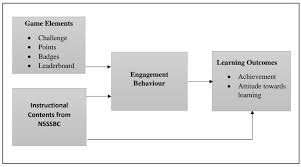
\includegraphics[width=0.8\textwidth]{figures/gamefield.jpeg}
    \caption{Механик, динамик ба үр дүнгийн хамаарлын загвар}
    \label{fig:mechanics-dynamics-outcome}
\end{figure}

Энэ урсгал нь геймификацийн дизайны гол алдааг илчилдэг: mechanics шууд business KPI-г өсгөнө гэж үзэх. Үнэндээ mechanics нь dynamics-ээр, dynamics нь psychological need ба experience-ээр дамжин зан үйлд нөлөөлдөг; эцэст нь л learning, performance, loyalty зэрэг үр дүн гардаг. Landers-ийн theory of gamified learning үүнийг тодорхой хэлбэрээр тайлбарласан бөгөөд Sailer нарын туршилт specific elements нь specific psychological effects үүсгэдгийг харуулсан.

%----------------------------------------------------------------------
\section{Геймификацийн механикийн харьцуулсан хүснэгт}
%----------------------------------------------------------------------

\begin{table}[H]
\centering
\caption{Геймификацийн механикуудын харьцуулалт}
\label{tab:mechanics-comparison}
\small
\begin{tabular}{|p{2cm}|p{2.5cm}|p{2.5cm}|p{2.5cm}|p{2.5cm}|}
\hline
\textbf{Механик} & \textbf{Зорилго} & \textbf{Сэтгэлзүйн механизм} & \textbf{Давуу тал} & \textbf{Сул тал / эрсдэл} \\ \hline
Оноо & Үйлдлийг тоон хэлбэрт оруулж progress visible болгох & Informational feedback, micro-reward, progress salience & Хялбар ойлгомжтой, immediate feedback өгнө & Quantity-ийг quality-ээс давуу болгож болзошгүй; score chasing \\ \hline
Шагнал & Desired behavior-ийг бататгах & Reinforcement, prediction, closure & Onboarding ба habit bootstrapping-д тустай & Overjustification, reward dependency, manipulation \\ \hline
Түвшин & Урт хугацааны progression ба identity өгөх & Competence signal, status, scaffolded mastery & Mid/long-term commitment нэмнэ & Grind, elitism, late-user discouragement \\ \hline
Achievement / badge & Milestone-г тэмдэглэх, competency-г харагдуулах & Recognition, competence affirmation, collection motive & Portfolio, signaling, micro-certification-д сайн & Badge inflation; бүх badge ижил үнэ цэнтэй биш \\ \hline
Challenge / quest & Effortful action ба learning task-г чиглүүлэх & Goal-setting, challenge-skill balance, meaning & Дээд чанарын engagement, flow боломжтой & Хэт амархан бол boredom, хэт хэцүү бол anxiety \\ \hline
Leaderboard & Social comparison, status competition бий болгох & Norm salience, competition, public recognition & Short-term activity spike өгч чадна & Shame, demotivation, cheating, bottom-rank dropout \\ \hline
Streak & Давтамжтай зуршил үүсгэх & Commitment, loss aversion, consistency identity & Habit formation-д хүчтэй & Missed day anxiety, unhealthy compulsion \\ \hline
Narrative / game fiction & Action-г утга учиртай context-д суулгах & Meaning, immersion, situated relevance & Behavioral outcomes-д эерэг moderator байж болно & Superficial theme бол novelty богино настай \\ \hline
Collaboration + competition & Social energy-г balancing хийх & Relatedness + competence зэрэг өдөөдөг & Competition alone-оос илүү тогтвортой байж болно & Team freeloading, conflict \\ \hline
\end{tabular}
\end{table}

Практикт хамгийн үр дүнтэй паттернууд дараах шинжтэй байдаг. Нэгд, micro-loop: үйлдэл $\to$ хурдан буцах холбоо $\to$ дараагийн achievable challenge. Хоёрт, meso-loop: module/quest/level progression. Гуравт, macro-loop: identity, career path, social standing, skill portfolio. Trailhead rank, Duolingo league + streak, Microsoft Learn achievements зэрэг системүүд энэ гурван түвшнийг өөр өөр хослуулдаг.

%----------------------------------------------------------------------
\section*{Эмпирик баримт, сэтгэлзүйн нөлөө, тайлбарлах механизм}
%----------------------------------------------------------------------

Геймификацийн empirical literature-ийн эрт үеийн системчилсэн тойм 2014 онд нийтлэгдэж, эерэг үр нөлөө ажиглагдах боловч тэдгээр нь контекст ба хэрэглэгчээс хүчтэй хамаардаг гэж дүгнэсэн. Энэ нь өнөөдөр ч үнэн хэвээр байна: геймификаци ``ажиллана'', гэхдээ ямар ч аудитори, ямар ч механик, ямар ч хугацаанд, ямар ч зорилгод ижил хэмжээгээр ажиллахгүй.

Суралцахуйн контекст дахь хамгийн хүчтэй тоон нотолгооны нэг нь Sailer ба Homner-ийн мета-анализ юм. Тэд gamification нь cognitive learning outcomes-д $g = .49$, motivational outcomes-д $g = .36$, behavioral outcomes-д $g = .25$ гэсэн жижиг боловч статистикийн хувьд ач холбогдолтой эерэг нөлөөтэйг харуулсан. Гэвч motivational ба behavioral effects нь high-rigor sub-split-д тогтворгүй байсан бөгөөд game fiction, social interaction, ялангуяа competition-ийг collaboration-тай хослуулах зэрэг moderator-ууд чухал байсан. Иймээс эффект хэмжээ нь байгаагаараа чухал, гэхдээ ``хэрхэн gamify хийх вэ?'' гэдэг асуулт ``gamify хийх үү?'' гэдгээс илүү чухал гэсэн үг.

Game-based learning ба serious games талд мөн ижил зураг харагддаг. Wouters нар serious games нь conventional instruction-оос learning ба retention талд давуу байж болохыг харуулсан бол Clark нар digital games and learning-ийн мета-анализдаа design features ба comparison conditions маш чухал буйг онцолсон. Өөрөөр хэлбэл ``тоглоом болгох'' нь дангаараа бус, тухайн тоглоом юу сургаж, яаж scaffold хийж, ямар feedback өгч, ямар comparison group-тэй харьцуулснаас үр дүн хамаарна.

Микро түвшний механизмын хувьд, individual elements ижил нөлөөтэй биш. Mekler ба хамтран зохиогчид points, levels, leaderboards нь performance quantity-ийг нэмэгдүүлсэн ч perceived competence эсвэл intrinsic motivation-ийг мэдэгдэхүйц өсгөөгүйг харуулсан. Харин Sailer нарын туршилтад badges, leaderboards, performance graphs нь competence satisfaction болон task meaningfulness-д; avatars, meaningful stories, teammates нь relatedness-д эерэг нөлөө үзүүлсэн. Энэ нь ``gamification per se'' бус ``specific elements have specific psychological effects'' гэсэн зарчмыг баталдаг.

Сэтгэлзүйн нөлөөний талаас геймификаци нь эерэг ба сөрөг аль алиныг үүсгэж болно. Эерэг талд competence, progress visibility, attention focus, persistence, social belonging, meaning, self-efficacy, habit consistency өсөх боломжтой. Сөрөг талд controlling rewards, social comparison pressure, shame, novelty decay, leaderboard fatigue, missed-streak anxiety, random reward compulsion, quantity-over-quality distortion үүсч болно. Extrinsic rewards intrinsic motivation-ийг ялангуяа completion-contingent ба expected tangible reward нөхцөлд бууруулах эрсдэлтэйг Deci, Koestner, Ryan-ийн мета-анализ эртнээс харуулсан.

Flow ба immersion-ийн талаас challenge--skill balance нь flow-ийн чухал antecedent боловч цорын ганц нь биш; clear goals ба sense of control мөн хүчтэй хувь нэмэртэй. Jennett нар immersion-ийг subjective questionnaire, task completion time, eye movement зэрэг субъектив ба объектив хэмжүүрээр зэрэг хэмжиж болдгийг харуулсан; мөн immersion үргэлж ``таатай'' биш, заримдаа anxiety ба uneasiness өндөр байж болно. Brown ба Cairns immersion-ийг engagement, engrossment, total immersion гэсэн шаталсан үйл явц гэж үзсэн нь design diagnosis хийхэд одоо ч хэрэгтэй.

%----------------------------------------------------------------------
\section*{Оролцоо ба immersion-ийг хэмжих үзүүлэлтүүд}
%----------------------------------------------------------------------

Геймификацийн хэмжилтэд хамгийн нийтлэг алдаа нь ганц KPI-гаар амжилтыг дүгнэх явдал юм. Time-on-task, session length, dwell time зэрэг behavioral metrics нь хэрэгтэй боловч утга нь хоёрдмол: урт хугацаа нь өндөр engagement ч байж болно, эсвэл төөрөгдөл, муу usability-ийн шинж ч байж болно. Иймээс behavioral, psychological, experiential, learning/performance, social, ethical metrics-ийг хамтад нь харах шаардлагатай.

Хэрэглэгчийн оролцоог хэмжихэд UES ба UES-SF хамгийн ашигтай стандартуудын нэг. Original UES нь aesthetic appeal, focused attention, novelty, perceived usability, felt involvement, endurability гэсэн зургаан хэмжээсээр 31 зүйлтэй байсан; дараа нь refined analysis-ээр short form гарч, дөрвөн хүчин зүйлийн бүтэц баталгаажсан. Энэ нь retention-ийг тайлбарлах survey layer болж өгдөг.

Тоглоомын engagement ба immersion-д GEQ, immersion questionnaire, Flow State Scale, GAMEFULQUEST, GAMEX зэрэг хэрэгслүүд ашиглагддаг. GEQ нь video game-playing дахь engagement-ийг psychometrically strong хэмжүүр болохыг Brockmyer нар харуулсан. Flow State Scale нь optimal experience-ийн олон хэмжээсийг барьдаг; GAMEFULQUEST ба GAMEX нь gamified systems дахь perceived gamefulness-ийг хэмжихэд зориулагдсан.

Сэдэлийн түвшинд IMI, basic psychological need satisfaction, self-efficacy, expectancy-value survey, perceived challenge/skill balance асуулга хэрэгтэй. Хэрэв бүтээгдэхүүн ``сурахад'' чиглэсэн бол learning outcome, transfer, retention, delayed recall, quality score-г; ``ажилд'' чиглэсэн бол task accuracy, speed, repeat usage, skill verification, error reduction-г; ``engagement app'' бол D1/D7/D30 retention, reactivation, challenge completion, churn after failure-г хамт хэмжих ёстой.

Immersion/flow-ийн объектив метрик нь eye movements, switch-cost task, task interruption cost, физиологийн ачаалал, self-report-тай triangulation хийх үед илүү үнэ цэнтэй. Практик measurement dashboard дараах бүтэцтэй байвал тохиромжтой: Acquisition (activation, onboarding completion); Engagement (focused attention, challenge completion, repeat visits); Immersion (flow score, interruption sensitivity, time distortion); Motivation (IMI, need satisfaction, self-efficacy); Learning/performance (quiz accuracy, transfer, retention); Ethics (pressure, shame, compulsive return, overspending-like behavior, unfairness perception).

%----------------------------------------------------------------------
\section*{Практик жишээ ба кейсүүд}
%----------------------------------------------------------------------

Бодит платформуудын жишээ нь механик хэрхэн багцлагддагийг сайн харуулдаг. Доорх кейсүүдийг ``үр дүн баталгаатай загвар'' гэж бус, ``design pattern-үүдийн бодит хэрэгжилт'' гэж унших нь зөв. Тэдгээрийн заримд official product documentation, заримд нь independent/academic evidence хавсарна.

\textbf{Боловсролын кейс.} Kahoot! нь game-based response system-ийн жишээ. 93 судалгааны тоймд Kahoot! нь learning performance, classroom dynamics, attitudes, anxiety дээр ерөнхийдөө эерэг нөлөөтэй гэж дүгнэсэн. Гэхдээ time stress, losing-оос айх, hard to catch up, network problems, projected-screen readability, хурд дээр суурилсан scoring нь reflection-ийг бууруулах эрсдэлтэй гэж мөн тэмдэглэсэн. Эндээс харахад ``classroom energy'' өсөх нь дангаараа сайн дизайн биш; таймер, scoring, retry, peer pace support-ийг маш болгоомжтой тааруулах ёстой.

\textbf{Аппын кейс.} Duolingo нь streak, XP, leagues, friend streak, crowns/gems зэрэг олон механикийг нэгтгэсэн хамгийн өргөн танигдсан жишээний нэг. Official materials-д leagues нь weekly XP дээр суурилж promotion/demotion хийдэг, friend streak нь хоёр тал хоёулаа өдөр бүр lesson хийж байж хадгалагддаг, efficacy report-д beginning-level course completers нь reading proficiency дээр intermediate түвшинд хүрч, listening дээр novice түвшинд үлдсэн гэж мэдээлсэн. Энэ нь нэг чухал сургамж өгнө: gamified engagement metrics өндөр байсан ч learning outcomes нь domain-by-domain ялгаатай байж болдог. Тиймээс engagement feature-үүдийг skill outcome-оос салгаж хэмжих ёстой.

\textbf{Корпорацийн сургалтын кейс.} Salesforce-ийн Trailhead нь corporate learning gamification-ийн canonical pattern юм. Official docs-д modules/projects completion нь badges ба points өгч, тэдгээр нь Trailblazer Rank рүү хуримтлагддаг гэж тайлбарласан; profile дээр rank, badges, earned points, trails completed харагддаг; үндсэн messaging нь ``learn new skills $\to$ get rewarded $\to$ rank up $\to$ showcase expertise'' гэсэн progression + signaling architecture юм. Энэ нь skill acquisition, credential signaling, social visibility, self-paced progression-ийг нэг системд холбосон корпоратив жишээ.

\textbf{Албан ёсны сургалтын экосистемийн кейс.} Microsoft-ийн Learn экосистемд achievements, badges, trophies, XP нь profile-based learning transcript ба achievements view-тэй холбогддог. Энэ нь gamification-ийг ``career-readable proof of progress'' хэлбэрт ашиглаж буй жишээ бөгөөд purely playful loop-оос илүү credential-oriented loop юм. Ийм системүүдэд badge/XP нь intrinsic fun-аас илүү self-efficacy, career relevance, public progress signaling-ээр ажиллах нь элбэг.

Эдгээр кейсүүдийн хөндлөн сургамж нь ижил. Боловсролын системүүд challenge, feedback, pacing дээр эмзэг; app системүүд streak, league, habit pressure дээр эмзэг; корпорацийн системүүд badge inflation ба signaling validity дээр эмзэг. Сайн дизайн гэдэг нь илүү олон mechanics нэмэх биш, харин domain-specific failure mode-ийг урьдчилан тооцоолохыг хэлнэ.

%----------------------------------------------------------------------
\section*{Шилдэг туршлага, ёс зүй, хэрэгжүүлэх шалгах хуудас}
%----------------------------------------------------------------------

Сайн геймификацийн үндэс нь aesthetics биш, alignment юм. Үйл ажиллагааны бодит үнэ цэнэ сул байхад game layer нэмэх нь богино хугацаанд novelty effect өгч болох ч урт хугацаанд decay хийнэ. Seaborn ба Fels-ийн тойм definitional inconsistency, weak theoretical grounding, mixed empirical findings, inadequate experimental design зэрэг асуудлыг эртнээс анхааруулсан. Тиймээс implementation-ийг ``feature shipping'' биш, theory-backed intervention гэж үзэх ёстой.

Ёс зүйн гол эрсдэлүүдийг дөрвөн блокт ойлгож болно:
\begin{enumerate}
  \item \textbf{Манипуляци ба compulsion:} variable/uncertain rewards, loss aversion, streak pressure-ийг хэт ашиглах.
  \item \textbf{Нийгмийн хор хөнөөл:} public leaderboard-оор ичгүүр, humiliation, chronic low-rank demotivation үүсгэх.
  \item \textbf{Суралцахуйн гажуудал:} point chasing-аас болоод reflection ба mastery буурах.
  \item \textbf{Predatory monetization-тэй төстэй загвар:} randomized rewards, loot-box-like complexity, ялангуяа эмзэг хэрэглэгчдэд хэт өдөөлт өгөх.
\end{enumerate}
Loot boxes-ийн талаарх судалгаанууд санамсаргүй шагналын механик нь consumer protection ба harm minimization талаас анхаарах шаардлагатайг онцолдог.

Best practice-ийн түвшинд дараах зарчмууд хамгийн тогтвортой. Meaningful core loop-гүй бол gamify хийх хэрэггүй. Early stage-д confidence-building success өг, mid stage-д adaptive challenge өг, late stage-д identity ба mastery signaling өг. Competition-ийг collaboration-тай тэнцвэржүүл. Badges-ийг competency evidence-тэй холбо, зүгээр цуглуулах тэмдэг болгож бүү сулруул. Metrics-ээ retention-оор хязгаарлахгүй, motivation, immersion, learning quality, ethics indicators-тай хослуул. Failure-ийг shame бус informative feedback болгон хувирга.

\textbf{Хэрэгжүүлэх шалгах хуудас:}
\begin{enumerate}
  \item Үндсэн зорилгоо тодорхойл: engagement уу, learning үү, performance уу, loyalty юу. Нэг системд бүгдийг зэрэг зорих бол KPI conflicts-ийг урьдчилан тодорхойл.
  \item Desired behavior chain-аа зур: ямар үйлдэл $\to$ ямар intermediate behavior $\to$ ямар final outcome.
  \item Хэрэглэгчийн сегмент бүрт early skill, confidence, social preference, competition tolerance-ийг тодорхойл. Demographic differences ба novelty decay боломжтойг тооц.
  \item Нэг mechanics-ийг нэг psychological purpose-тэй холбо: points = feedback, badges = recognition, levels = progression, challenges = mastery, streak = consistency. Нэг механикт олон зорилго ачихгүй.
  \item Challenge--skill balance, clear goals, immediate feedback-ийг MVP түвшинд шийд. Flow-г cosmetics-оор биш task design-аар бүтээ.
  \item Competition-ийг зөвхөн top performers-д биш, team-based, bracketed, opt-out, self-referenced mode-оор хувилбаржуул.
  \item Survey + analytics + outcome measures гэсэн гурвалсан хэмжилт хэрэглэ. UES, IMI/need satisfaction, learning/performance metrics-ийг хамтад нь ав.
  \item A/B test хийхдээ novelty window, long-term decay, after-reward drop-off, post-failure churn-ийг заавал шалга.
  \item Ethical guardrail тогтоо: streak loss protection, private mode, leaderboard opt-out, probability disclosure, no surprise monetization, vulnerable users protection.
  \item Feature launch-аас өмнө ``хэрэв энэ механик амжилттай ажиллавал хүмүүс илүү сайн сурах уу, эсвэл зүгээр илүү их дарах уу?'' гэсэн асуултад хариул.
\end{enumerate}

\end{sloppy}

%=============================================================================
% НЭМЭЛТ ОНОЛЫН ТОЙМ II: 
%=============================================================================

\subsection{Unity AR Foundation, ARCore, ARKit платформуудын харьцуулалт}
\begin{sloppy}

Энэхүү тайлан нь Unity-ийн AR Foundation, Google-ын ARCore, болон Apple-ийн ARKit платформуудын үзүүлэлт, давуу ба сул тал, хөгжүүлэлтийн ажлын урсгал, ба аялал жуулчлалд чиглэсэн AR хэрэглээнд (байршилд суурилсан AR, зайн мэдээллийн давхарга, навигаци, өгүүллэгийн түүх, бага сүлжээний нөхцөл зэрэг) тохирох байдалд хийсэн иж бүрэн харьцуулалт юм. Unity AR Foundation нь нэг цөм дээр хөгжүүлж Android болон iOS-д зориулсан AR апп бүтээх боломжийг олгодог иж бүрэн cross-platform хүрээ юм. ARCore, ARKit хоёр нь тус бүр Android ба iOS платформуудад нөлөөлөх SLAM болон компьютер харааны чадварыг ашиглан төхөөрөмжийн байрлал, талбарийн илрүүлэлт зэрэг гол AR функцуудыг хариуцдаг. Ямар ч платформыг сонгосон ч гүйцэтгэл нь төхөөрөмжийн техник чадвар, зураг эсвэл сенсорын чанар, платформын дэмжлэгт ихээхэн хамааралтай байдаг. Unity AR Foundation нь эдгээр платформуудын аль алиныг хариуцдаг тул (дор үндсэндээ ARKit эсвэл ARCore-г дууддаг) кросс-платформ хөгжүүлэлтийн ихэнх цаг хугацааг хэмнэх боломжтой боловч платформ тус бүрийн төрөлжсөн функцууд (жишээ нь: ARKit-ын LiDAR сканнер болон Apple-ийн байршлын цэгүүд эсвэл ARCore-ын дэлхийн масштабын гео-анкор) бүгд дамжуулагдаад байдаггүй сул талтай.

Уг тайланд платформ тус бүрийн онцлогуудыг цуврал хүснэгтээр харьцуулж, аялал жуулчлалд зориулсан AR хэрэглээний жишээ болон шаардлагад нийцэх боломжийг үнэлнэ. ARCore-ын Геоспатиал API нь дэлхийн даяар байрлах бодит байршилд хүрээнд агуулга наах боломж олгодог. Харин ARKit-ын Location Anchors (ARGeoAnchor) нь тодорхой хотууд болон газар нутгуудад л байдаг (iOS 16+ гэсэн хязгаарлагдмал дэмжлэгтэй). Олон хэрэглэгчтэй хамтран ажиллах AR-д ARCore нь Cloud Anchors ашиглан олон Android, iOS төхөөрөмж дээр нэгэн зэрэг ижил объектуудыг байрлуулахаас гадна цаашид давтан холбогдох боломжийг олгодог. ARKit-д олон хэрэглэгчийн AR-г ARWorldMap ашиглан нэг орчинг бусад төхөөрөмж рүү дамжуулах замаар бий болгож байдаг.

%----------------------------------------------------------------------
\section{Платформуудын Харьцуулалт}
%----------------------------------------------------------------------

\textbf{Unity AR Foundation (Unity 3D).} Unity хөдөлгөөнт болон үл харагдах AR/MR/VR орчны хөгжүүлэлтийн иж бүрэн game engine юм. Түүний AR Foundation хэсэг нь Android, iOS, бас бусад XR төхөөрөмжүүдийг нэг кодын цөм дээр бүтээх боломж олгох cross-platform framework. AR Foundation нь өөрөө бие даасан AR алгоритм агуулаагүй ч платформ тус бүрийн (ARKit, ARCore, Magic Leap гэх мэт) онцлог API-г нэгэн интерфэйстэй уялдуулан ашигладаг. Тиймээс Unity AR Foundation төсөлд шаардлагатай AR компонентуудыг (Plane Detection Manager, Raycast Manager гэх мэт) оруулж өгснөөр, төслийг ямар гар утсан дээр ажиллуулахыг сонгож суулгалтыг тохируулна. Баригдсан үед iOS дээр ARKit, Android дээр ARCore-ын дохиоллыг дуудахаар холбогдсон тул нэгэн кодыг ашиглан хоёуланд бүтээж чадна. Unity AR Foundation нь Asset Store, визуал хөгжүүлэлтийн хэрэгслийг ашиглах боломжтой, мөн C\# дээр программчилна.

\textbf{ARCore (Google).} Google-ын хөгжүүлсэн Android (ба тодорхой тооны iOS) хөндлөн платформ SDK. ARCore голчлон ARCore SDK (Android) болон ARCore Extensions зэрэг тусгай сангуудыг агуулна. ARCore нь Motion Tracking, Planes, Depth API, Light Estimation зэрэг үндсэн AR боломжуудыг хангадаг. Төхөөрөмжийн камерын дүрс ба IMU мэдээллийг нэгтгэж VIO ашиглан SLAM хийдэг. ARCore нь олон Android утасны платформд (Android 7.0 ба түүнээс дээш) дэмжигддэг боловч зөвхөн ARCore гэрчилгээтэй загваруудад ажиллана. ARCore-ийн нэмэлт Геоспатиал API нь Google Street View 3D загварт тулгуурлан дэлхийн хаанаас ч амжилттай байршил тогтоох боломж олгодог. ARCore-ийн SDK нь Java/Kotlin (Android), C\# (Unity AR Foundation), C++ (NDK) хэл дээр ашиглаж болно. Чухал давуу тал нь Cloud Anchors ашиглан олон хэрэглэгчид хоорондын AR-хамтын туршлагыг бий болгох боломжтой. ARCore SDK нь үнэгүй.

\textbf{ARKit (Apple).} Apple-ийн iOS/iPadOS аппарат дээр ажиллах AR-т зориулсан дэлхийн стандарт SDK. ARKit нь төхөөрөмжийн камер, IMU-гаас гадна дэвшилтэт төхөөрөмжид LiDAR сканнер, TrueDepth камер зэрэг нэмэлт сенсор ашиглан өргөн хүрээний SLAM-тэй. ARKit-ын гол боломжууд: World Tracking (6DOF байршлын хяналт), Visual-Inertial Odometry, Plane Detection (хэвтээ/босоо тэнхлэгийн гадаргуу илрүүлэх), Depth Mapping, Light Estimation, Image/Object Detection, Face Tracking (TrueDepth) зэрэг багтдаг. ARKit 2 (iOS12) болон түүнээс хойших хувилбарууд нь ARWorldMap ашиглан орчныг хадгалах, бусад төхөөрөмжид шилжүүлэх замаар олон хэрэглэгчийн AR-г дэмждэг. ARKit нь зөвхөн iOS төхөөрөмжүүд дээр ажиллах тул iOS 11.0 эсвэл түүнээс хойш, A9 ба түүнээс дэвшилтэт процесстэй утаснуудыг дэмжиж эхэлсэн.

%----------------------------------------------------------------------
\section*{Концептуал давуу ба сул талууд}
%----------------------------------------------------------------------

\textbf{Жишиг мэдлэг (SLAM/байршил тогтоох).} ARCore, ARKit аль аль нь VIO аргыг ашиглан төхөөрөмжийн байрлал, чиглэлийг тогтмол шинэчилдэг. Эдгээр нь камераар илэрч буй онцлог цэгүүдийг (feature points) барьж, хөдөлгөөний мэдээлэлтэй (accelerometer+gyroscope) уялдуулж бодит орчин дэх төхөөрөмжийн байрлалыг бодитоор тогтооно. Plane илрүүлэлт аль аль SDK-д байдаг. Гэсэн ч усан хөрстэй тэгш гадаргуу, тод бүтэцгүй хананд plane илрэхгүй байх зэрэг хязгаарлалт адилхан тул объектын байрлал тогтворгүй байж болно. ARCore нь илрүүлсэн feature цэгээр depth map үүсгэж, виртуал объектуудын бодит мөргөлдсөн байдал, гүн харагдах байдлыг сайжруулдаг. ARKit нь зарим шинэ iOS төхөөрөмжид Deep Fusion LiDAR ашиглан илүү нарийвчлалтай нүдэлцэх өөрчлөлтийг нэгтгэж чаддаг.

\textbf{Газарзүйн контент (геолокац, POI).} Аялал жуулчлалд газрын зураг, координатын систем, POI мэдээлэл хамгийн чухал. ARCore-ийн Geospatial API нь Google Street View 3D загвартай автоматаар нийцэж ажиллана. Энэ нь GPS-ийн нарийвчлалыг сайжруулж, дэлхий даяар газар зүйн координатын дагуу виртуал агуулга байрлуулах боломжийг олгоно. ARKit 6-ын Location Anchor нь одоогоор тодорхой хот суурин (Торонто, Сингапур, Сидней г.м.)-д л бий, ирээдүйд Apple Maps-тай холбогдох боломж нэмэгдэх хандлагатай байна.

\textbf{Олон хэрэглэгчийн AR.} Олон хэрэглэгчид зэрэг AR туршлагыг хуваалцахад ARCore болон ARKit хоёул боломжтой боловч стратеги нь өөр. ARCore нь Cloud Anchors API ашиглан үүлэн орчинд анкоруудыг хадгалж, бусад хэрэглэгчдэд давтан суулгах боломжийг олгодог. ARKit-д ARWorldMap дамжуулж (Multipeer Connectivity-ээр) нэгэн орчинд олон хүнд ижил тэгш координатын талбарыг ашиглах боломж бий. Ерөнхийд нь ARCore-ын олон төхөөрөмжийн дэмжлэг нь платформ хооронд (Android$\leftrightarrow$iOS) байдаг ба Cloud Anchors нь Google Cloud-д тулгуурладаг (интернет шаардлагатай) бол ARKit нь локал iCloud/Multipeer шийдэл дээр төвлөрдөг (зөвхөн Apple төхөөрөмжүүд хоорондод).

\begin{table}[H]
\centering
\caption{AR платформуудын иж бүрэн харьцуулалт}
\label{tab:ar-platform-full}
\small
\begin{tabular}{|p{3cm}|p{3.5cm}|p{3.5cm}|p{3.5cm}|}
\hline
\textbf{Үзүүлэлт / Платформ} & \textbf{Unity (AR Foundation)} & \textbf{ARCore (Android)} & \textbf{ARKit (Apple iOS)} \\ \hline
Дэмжих платформ & Android, iOS (нэг код) & Android (7.0+, ARCore гэрч.) & iOS (iOS 11+, A9+ утас) \\ \hline
Програмчлал & C\# (Unity) & Java/Kotlin (Android) & Swift/ObjC (iOS) \\ \hline
Мөрөнд байрлал & Боломжтой (ARKit/ARCore) & Боломжтой (VIO SLAM) & Боломжтой (VIO SLAM) \\ \hline
Plane илрүүлэх & Тийм (дэд бүрд ARKit/ARCore) & Тийм & Тийм \\ \hline
Зурган таних & Тийм & Тийм & Тийм \\ \hline
Face Tracking & Тийм (лидөө ARKit дээр) & Хязгаарлагдмал & Тийм (TrueDepth) \\ \hline
Depth мэдрэх & Тийм (LiDAR/Depth API) & Тийм (Depth API) & Тийм (LiDAR/dual cam) \\ \hline
Геолокац/Анкор & Тийм (ARCore/ARKit функц) & Боломжтой (Geospatial) & Хязгаарлагдмал (Location Anchors) \\ \hline
Олон үйлчлэгч & Тийм (Cloud/WorldMap) & Тийм (Cloud Anchors) & Тийм (WorldMap/Multipeer) \\ \hline
Лиценз & Personal үнэгүй; Pro \$1800/жил & Чөлөөт SDK & Чөлөөт SDK; Apple dev \$99/жил \\ \hline
Хамгийн тохирох & Cross-platform AR (Android+iOS) & Android-д зориулсан AR, гео-апп & iOS-д зориулсан өндөр чанарын AR \\ \hline
\end{tabular}
\end{table}

%----------------------------------------------------------------------
\section*{Аялал жуулчлалын AR-д зориулсан тохиромжит боломжууд}
%----------------------------------------------------------------------

\textbf{Байршилд суурилсан интерактив туршлага.} Төрөл бүрийн газарзүйн POI-д мэдээлэл давхарлахад GPS/геолокацийн функц чухал. ARCore-ийн Geospatial API нь Google Street View-ийн өргөн үүлэн зураглалд тулгуурлаж дэлхийн өнцөг булан бүрт виртуал контент байрлуулах боломжтой. Unity/AR Foundation + ARCore Extensions хослол хэрэглэвэл Google VPS-ийг Unity апптай нэгтгэж ашиглаж, улаан таслалгүй дэлхий даяар AR мэдээлэл дамжуулах боломжтэй. ARKit-ын Location Anchors нь өнөөгийн байдлаар цөөн хэдэн хотод байдаг тул томоохон хотын чиглэлд болон зурагт дээрх бодит байршлыг тусгаж өгөхөд хэрэглэгддэг. Судалгаагаар аялалд зориулсан AR аппликейшнүүд нь байршлын активчлал (GPS-geofence дөхөх үед агуулга нээгдэх) аргыг өргөн ашигладаг.

\textbf{POI давхарга, түүхийн өгүүллэг.} Аяллын туршид дурсгалын газрууд дээр мэдлэг, мультимедиа өгүүлэхэд AR ашиглагдана. Энэ нь байрлал дээр тулгуурласан интерактив дэлгэц (монументын нүүрэн дээр харагдах текст, 3D дүрс гэх мэт) хэлбэрээр, эсвэл тойргийн навигациар (туршилтын маршрутад AR тэмдэг тавих) хэрэглэгддэг. ARKit ба ARCore хоёул камерыг ашиглан дүрс таних, объект таних боломжтой. Unity-гийн XR Interaction Toolkit-ийн тусламжтайгаар хэрэглэгч дэлгэцээр дарж зүйлсийг сонгох буюу эргүүлэх зэрэг интерактив боломжуудыг нэмнэ.

\textbf{Навигаци ба зааварчилгаа.} Хот дотор AR зам заагч (шилэн тэмдэг), эсвэл хүрэх газар руу заасан виртуал сум/мөр үүсгэхдээ AR Foundation дээр raycast ашиглана. ARCore Гео API нь GPS-гийн алдааг сайжруулж, гудамжны дагуу 3D зааврууд зааж өгөх боломж нэмдэг. ARKit-д Location Anchor ашиглан тухайн газрын харуулдаг эсвэл LiDAR map ашиглан.

\textbf{Бага сүлжээний нөхцөл.} Холболт муутай үед offline байдлаар орчны SLAM-ийг үргэлжлүүлэн ашиглаж болно, гэхдээ онлайн API (Geospatial, Cloud Anchor) ашиглагдахгүй. Газар зүйн байршилтай холбоотой гео-анкорууд, үүлэн сервис шаардлагатай зүйлс offline горимд боломжгүй, харин Unity+AR Foundation доторхи суурь зураглал/plane-detection/games гэх мэт мэдээлэл төхөөрөмж дээрээ байна. Том агуулгыг орон нутгийн санах ойд хадгалах, bааз (offline map) бий болгох шийдлийг төлөвлөх боломжтой.

%----------------------------------------------------------------------
\section*{Гүйцэтгэл, SLAM, дүрслэлийн тогтоолт}
%----------------------------------------------------------------------

\textbf{Динамик чадварын ялгаа.} Unity AR Foundation нь зарим overhead дагуулна (Unity Engine), харин Unity-ийн шинэчлэгдсэн render pipeline (URP) AR-д тохиромжтой. ARCore нь ихэвчлэн Qualcomm Snapdragon платформ дээр сайн ажиллах чадвартай бөгөөд ARCore гэрчилгээтэй утастай байдаг. Android-ын хувьд рам багатай эсвэл өндөр нягтаршилтай дэлгэц зарим AR сцэнарт асуудал үүсгэж болно. ARKit нь Apple Silicon чипүүд (A-сери) дээр оновчтой, бүх iPhone/iPad-н чадлыг нэг стандарт хэлбэрт оруулсан.

\textbf{SLAM, дүрслэлийн хяналт.} ARCore, ARKit аль аль нь 6DOF төхөөрөмжийн байрлал болон орчин таних (planes, feature points) боломжуудтай. ARCore нь ``visual and inertial data''-г нэгтгэн SLAM хийдэг гэж баримт бичигт тайлбарласан; тэгээд ARCore нь давхарга (plane), feature points ашиглан объект байрлуулах боломжийг гаргадаг. ARKit дээр ``World Tracking'' нь төхөөрөмжийн байрлал, чиглэлийг хангалттай үнэн зөвөөр баталгаажуулж өгдөг бөгөөд энэ нь хэвтээ, босоо хавтгайг илрүүлж өгдөг.

\textbf{Сенсорын хандалт.} ARCore нь зураглаач камерыг, акселерометр, гироскоп болон зарим төхөөрөмжид Depth API зэрэг нэмж гүн мэдээллийг ашигладаг. ARKit нь TrueDepth камертай (iPhone X ба түүнээс хойшх) нүүрний барихад, LiDAR сканнертай (зарим iPad Pro, iPhone 12/13 Pro) дотоод орчныг илүү нарийвчлан зураглахад дэмжлэг үзүүлдэг.

\textbf{Орчны хадгалалт (Mapping/Persistence).} ARCore SDK-д орчинд анкор байршуулах функц суулгаж, Cloud Anchors ашиглан үүлэн дурсамж хийнэ. Энэ нь тухайн орчинд виртуал объектыг удаан хугацаанд хадгалах боломжийг олгодог. ARKit-д ARWorldMap ашиглан тухайн сессийн бүх ойлголтыг нэг объектыг болгож архиважуулж, хүссэн үедээ сэргээх боломжтой. Оффлайн хадгалалтын хувьд ARKit-д ARWorldMap-ийг файл болгоод нөхцөлд ашиглаж, Unity-д AR Session Recording \& Playback (4.x+) ашиглан турших боломжтой. ARCore нь Cloud Anchors ашиглах шаардлагатай (интернет зайлшгүй).

%----------------------------------------------------------------------
\section*{Хөгжүүлэлтийн ажлын урсгал, тоног хэрэгсэл, Asset Pipeline}
%----------------------------------------------------------------------

\textbf{Үйл явцын давталт.} AR аппликейшн хөгжүүлэхэд Agile/iterative аргыг түгээмэл ашигладаг. Учир нь AR нь орчинд шууд холбогдсон технологи тул прототипийг биечлэн хэрэгжүүлж, утас дээр туршиж, шаардлагатай удаа сайжруулах хэрэгтэй болдог. Unity-д хөгжүүлэгчид Play Mode дотор энгийн өмнөх зураглал, plane detection-ийг шалгаж туршиж чаддаг. AR MARS гэх мэт нэмэлтүүдийг ашигласнаар бодит орчинд аргачлал гаргахад туслана. ARCore/ARKit native-д хөгжүүлэхэд төхөөрөмж дээр шууд apk эсвэл ipa үүсгээд турших шаардлагатай тул iteration жаахан удаан байж болох юм.

\textbf{Төгсөх шалгалт, төхөөрөмж дээр суулгах.} Аль ч платформд арын камера, хөдөлгөөн мэдрэгчийн мэдээллийг ашиглахаас гадна боломжит бүх төхөөрөмж дээр шалгаж үзэх шаардлагатай. Unity Cloud Build, Jenkins, GitHub Actions зэрэг CI/CD нь Unity болон native төслүүдийг автоматаар эвлүүлэхэд тусална. Мөн Device Farms (Firebase Test Lab, Apple TestFlight гэх мэт) бүрэн хэмжээлсэн тест хийхэд ашиглагддаг.

\textbf{Агуулахын (Asset) урсгал.} Unity-т 3D загвар (FBX, OBJ, GLTF), видео, аудио гэх мэт агуулгыг Asset Store эсвэл өөрөөсөө оруулж ашиглах хялбар. ARCore/ARKit native-д SceneKit (USDZ) эсвэл OpenGL/Metal рендерлэлт, ARMedia гэх мэт файлуудыг оруулна. Content management систем ашиглах замаар Unity эсвэл native апп руу динамик агуулга татах боломжтой.

\textbf{CI/CD, өгөгдлийн хуваалцалт.} Unity Build Automation, Fastlane (iOS), Gradle (Android) зэрэг системээр тогтмол суулгац бүтээдэг. Unity Cloud Build нь олон платформд зэрэг гүйцэт бүтээхэд тохиромжтой, харин native төслүүдэд тус бүрийн үйлчилгээгээ хэрэглэх шаардлагатай.

%----------------------------------------------------------------------
\section*{Backend интеграц, газрын зураг, агуулгын менежмент}
%----------------------------------------------------------------------

\textbf{Газрын зураг болон байршилын API.} Google Maps/Geocoding API, Mapbox, OpenStreetMap, Apple MapsKit гэх мэт үйлчилгээнүүд байршлыг тодорхойлж холбоход хэрэг болно. ARCore Гео API нь Google VPS-тэй тул Google хэрэглэх шаардлагатай. ARKit Location Anchors нь Apple Maps-тай шинэчлэгдэж ажиллана. POI дата, гудамжны зураглалд Google, Mapbox, HERE зэрэг үйлчилгээ ашиглаж болно.

\textbf{Үүлэн болон Оролтын үйлчилгээ.} ARCore Cloud Anchors нь Google Cloud-т онцгой ID үүсгэж хадгалдаг. ARKit хувьд iCloud дээр суурилсан ARWorldMap-ыг цааш дамжуулж болно. Мөн Microsoft Azure Spatial Anchors, Niantic Lightship гэх мэт олон платформ хянах боломжууд бий.

\textbf{Агуулгын сервер.} Өгөгдлийг хадгалах барилга, түүхийн текст, мультимедиа, 3D загвар зэргийг удирдах CMS-ууд (WordPress, Drupal, Strapi гэх мэт) баримт бичиг, видео, 3D файлыг сервер дээр хадгалж, AR апп руу хүснэгтээр дуудна. Туршилтын хувьд эдгээр нь RESTful эсвэл GraphQL API-гаар дамждаг.

%----------------------------------------------------------------------
\section*{Хөгжүүлэгчийн экосистем, баримт бичиг, лиценз}
%----------------------------------------------------------------------

\textbf{Unity AR Foundation.} Unity Technologies-гийн дэмжлэгтэй, иж бүрэн баримт бичиг, жишээ төслүүд, форум (Unity Answers, Discord) бий. Unity Asset Store дээр олон AR/DigitalTwin прототип байдаг. Лиценз нь жижиг компаниудад үнэгүй, Unity Pro нь ~\$1800/жилд. AR Foundation нь идэвхтэй хөгжиж байгаа, үе шатууд (4.x, 5.x, 6.x) гардаг.

\textbf{ARCore.} Google-ийн ARCore нь Android-д төвлөрсөн, тухайлбал Pixel, Samsung, Huawei гэх мэт ARCore-г дэмжсэн олон утсанд нэвтэрнэ. Техникийн баримт бичиг нь Google Developers сайтад сайн тайлбарлагдсан, pример кодууд (codelab, GitHub) олон. Лиценз үнэ төлбөргүй.

\textbf{ARKit.} Apple-ийн ARKit нь зөвхөн iOS хөгжүүлэгчдэд ээлтэй. Apple Developer сайтанд зохион байгуулалттай, WWDC видео, загварууд (sample projects) байдаг. Лиценз үнэгүй (зөвхөн жил бүрийн Apple Developer гишүүнчлэл \$99 шаардагдана). Apple нь ARKit-ын шинэчлэл тус бүрт AR туршлагын чанарыг сайжруулах түлхүү анхаарал тавьдаг (LiDAR, хуваалцсан туршлага, Vision Pro).

\textbf{Платформын ирээдүйн чиглэл.} Unity AR Foundation нь одоо VisionOS (Apple Vision Pro) дэмждэг болсон; ирээдүйд ямар ч XR platform-т Unity дамжлага болно. ARCore нь Geospatial API-г дэлхийд түгээж, гэрэлтүүлгийн шинэчлэл, ARCore Extensions-ээр олон шинэ боломжыг судалсаар байна. ARKit нь iOS шинэчлэлт бүрээр шинэ Location Anchor хотууд, өөрчлөлттэй түүхийн урамшуулал, enterprise зориулалттай RealityKit шинэчлэлүүд гаргаж байна.

\begin{figure}[htbp]
    \centering
    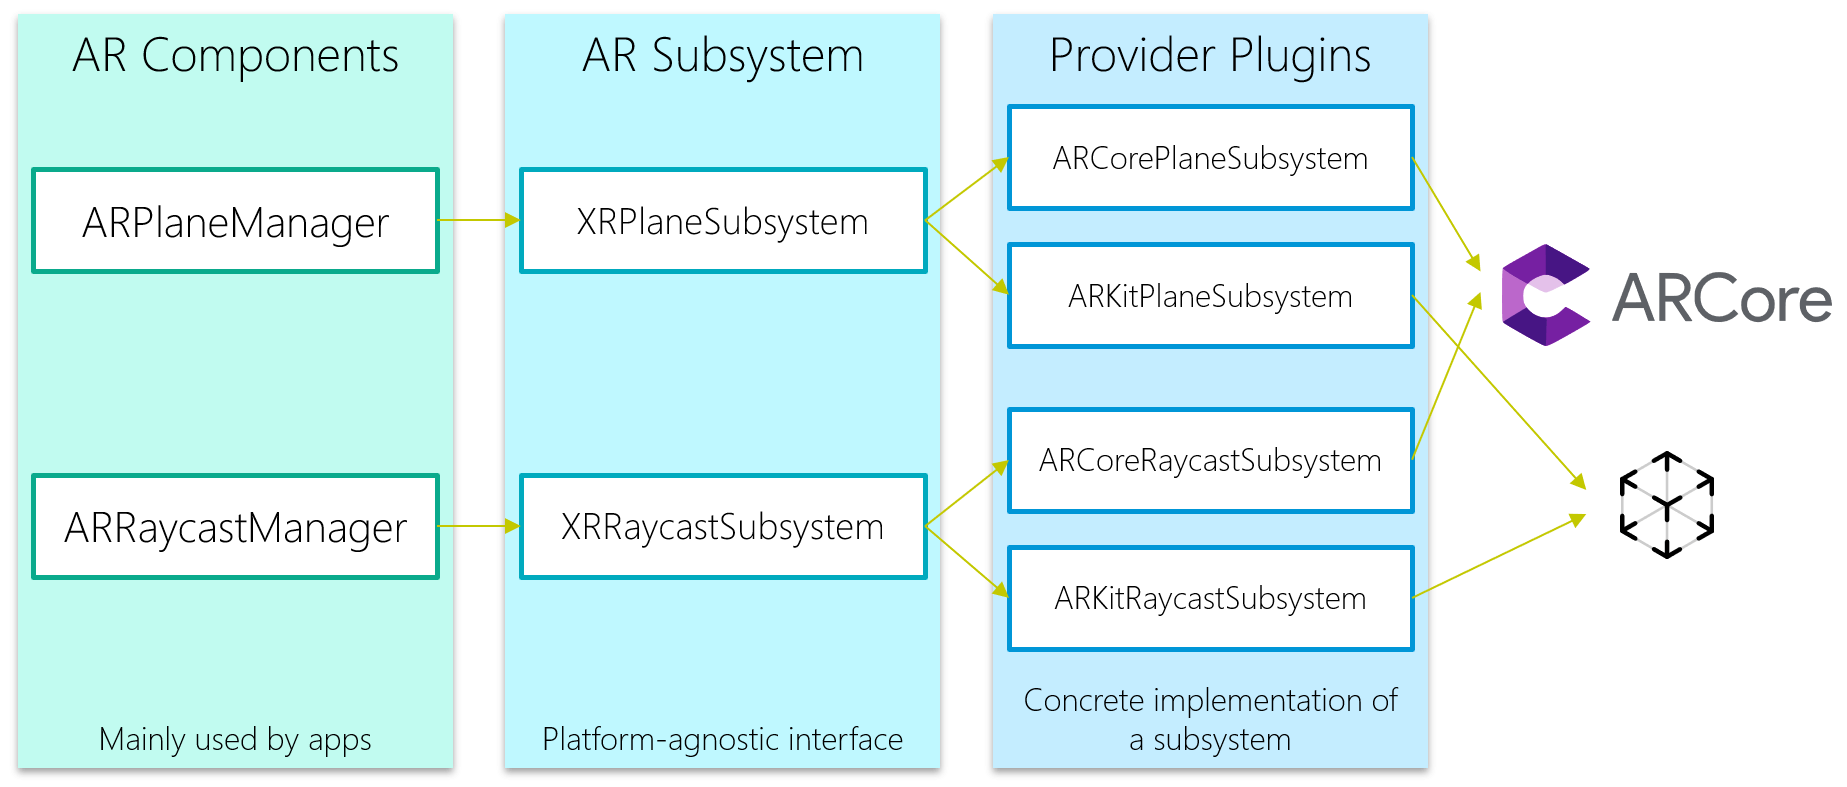
\includegraphics[width=0.8\textwidth]{figures/architecture.png}
    \caption{Unity AR Foundation-ын архитектур}
    \label{fig:ar-foundation}
\end{figure}

Unity AR Foundation-ын дэд бүтцийг харуулсан архитектурын ерөнхий зураг. Unity-ийн AR Foundation нь Apple ARKit XR Plugin болон Google ARCore XR Plugin-тай холбогдож, iOS ба Android төхөөрөмжүүд дээр ARKit болон ARCore-ийн SDK-уудыг харуулна. Мөн Cloud Anchors \& Geospatial API (Google VPS) болон газрын зургийн үйлчилгээ (Google Maps, Apple Maps) зэрэг серверийн үйлчилгээстэй холбогдож, байршилтай холбоотой агуулга байрлуулах боломж олгодог.

\end{sloppy}

%=============================================================================
% НЭМЭЛТ ОНОЛЫН ТОЙМ III: МОБАЙЛ AR АЯЛАЛ ЖУУЛЧЛАЛЫН СИСТЕМИЙН АРХИТЕКТУР
%=============================================================================

\section{Нэмэлт онолын тойм III: Мобайл AR аялал жуулчлалын тоглоомын систем дизайны онолын тойм}
\begin{sloppy}

\section*{Гүйцэтгэх хураангуй}

Мобайл AR аялал жуулчлалын тоглоомын үндсэн инженерчлэлийн асуудал нь ``газрын зураг дээр 3D объект харуулах'' асуудал биш, харин локал AR поз ба глобал геопозицийг нэгэн зэрэг зөв удирдах асуудал юм. GPS/GNSS нь хэрэглэгчийн глобал байршлыг өгдөг боловч ухаалаг утас нээлттэй тэнгэрийн дор ч түгээмэлдээ ойролцоогоор 4.9 м радиустай алдаатай байж, барилга, гүүр, мод, multipath ойлт зэрэг нөлөөгөөр улам мууддаг. Харин ARCore/ARKit төрлийн стекүүд камер ба IMU-д суурилсан хөдөлгөөн мөрдөлт, world tracking, plane detection, anchor зэргээр локал орчинд илүү тогтвортой AR байрлал тогтоодог. Иймээс сайн архитектур нь географийн trigger давхаргыг визуал/инерцийн бэхэлгээ давхаргаас тусгаарлах ёстой.

Платформ тодорхойгүй үед хамгийн зөв чиглэл нь capability-based, degradation-friendly архитектур юм. Android талд тодорхой мэдрэгч заавал байх албагүй, runtime detection болон optional feature gating хэрэгтэй; iOS/ARKit талд ч зарим чадамж нь зөвхөн LiDAR-тэй төхөөрөмжид идэвхтэй байдаг. Иймээс клиент талд нэг ``AR session orchestration'' давхарга байрлуулж, мэдрэгчийн бэлэн байдал, геолокацийн нарийвчлал, камераас шалтгаалах AR tracking quality, cache-тай эсэх, сүлжээний чанар зэргийг хэмжин тухайн мөчийн тоглоомын горимыг сонгодог байх нь зөв.

Газрын зураг ба геофенсийн давхарга нь хаана trigger өгөх асуудлыг шийддэг бол AR anchor/SLAM давхарга нь юуг яг хаана тогтоон дүрслэх асуудлыг шийднэ. Android geofencing нь fused location provider дээр сууж, батарейн үр ашгийг харгалзан загварчлагдсан; харин ARCore Geospatial API ба ARGeoAnchor зэрэг механизм нь WGS84 суурьтай глобал координатыг AR ертөнц рүү оруулж өгдөг. Тиймээс аяллын тоглоомын архитектур геофенсийг object placement-д бус, харин бүсийн trigger, prefetch, storyline activation-д ашиглах ёстой.

Контентын хувьд толгойгүй CMS, resource-oriented API, locale/fallback загвар, immutable asset bundle, CDN/edge cache, offline map cache-тай байх нь тоглоомын тогтвортой ажиллагаанд шийдвэрлэх нөлөөтэй. Судалгааны хувьд 2024 оны аялал жуулчлалын field experiment нь location-based AR нь хэрэглэгчийн шинэлэг мэдрэмжийг өсгөж болох ч замчилгааг хэт хатуу хийвэл орон зайн судлан тандах зан төлөвийг хязгаарлаж болзошгүйг харуулсан. Иймээс сайн систем нь контентыг нэг мөр маршрутаар хүчлэхээс илүү detour-tolerant, branchable, resume-capable байх ёстой.

Нууцлал, зөвшөөрөл, талбайн QA нь төслийн төгсгөлийн шалгалт биш, харин архитектурын эхний өдрөөс эхлэх ёстой. Байршил, камер, микрофон нь мэдрэмтгий өгөгдөлд хамаарах тул least privilege, progressive disclosure, approximate/reduced accuracy fallback, simulated route test, approximate-location test, AR session recording/playback, thermal monitoring зэрэг нь заавал системийн хэсэг байх ёстой.

%----------------------------------------------------------------------
\section*{Хамрах хүрээ ба суурь архитектурын зарчим}
%----------------------------------------------------------------------

Энэ тайлан нь тодорхой платформ, тоглоомын хөдөлгүүр, клауд вендор, лицензийн төсөв, зорилтот төхөөрөмжийн анги, нэгэн зэрэг идэвхтэй тоглогчийн тоо, хот/хөдөөгийн орчны төрөл, офлайн ашиглалтын түвшин, зохицуулалтын улс орон, контент модерацийн бодлогыг урьдчилан тогтоогоогүй нөхцөлд бичигдсэн. Иймд доорх дүгнэлтүүд нь концепцийн түвшний системийн дизайн бөгөөд ``which SDK is best'' гэсэн асуултад биш, ``ямар архитектурын хил зааг тавивал дараа нь өөрчлөлтөд тэсвэртэй байх вэ'' гэсэн асуултад хариулж байна.

Платформ тодорхойгүй үед гол зарчим нь ``native feature-ийг шууд бизнес логикт урсгахгүй, capability abstraction-аар дамжуулах'' юм. Android-ын албан ёсны мэдрэгчийн баримт бичиг төхөөрөмж бүр ижил sensor set-тэй байх албагүйг тодорхой хэлдэг бөгөөд runtime дээр sensor байгаа эсэхийг шалгаж feature-ээ асааж/унтраахыг зөвлөдөг; мөн manifest дээр sensor-оо үнэхээр зайлшгүй үед л required=true болгох хэрэгтэй гэж зөвлөдөг. ARKit талд ч LiDAR-тэй төхөөрөмжид л Depth API ба Instant AR идэвхждэг. Энэ нь ``device profile'' болон ``experience tier'' гэсэн ойлголтыг архитектурын төвд тавих ёстойг илтгэнэ.

\begin{figure}[htbp]
    \centering
    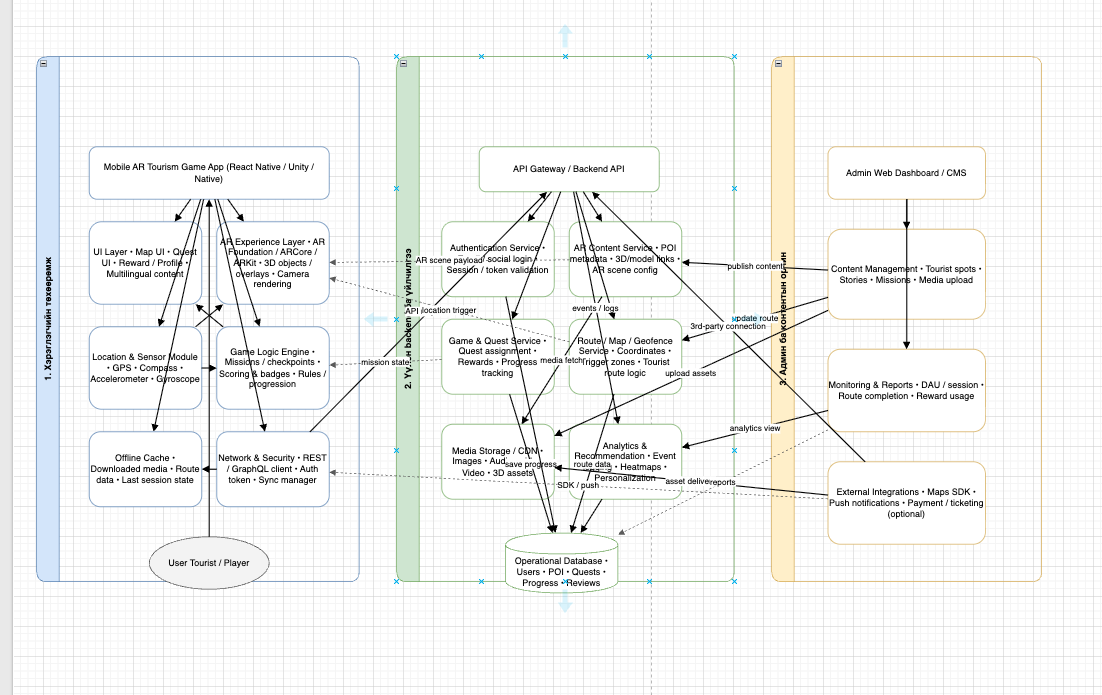
\includegraphics[width=0.8\textwidth]{figures/Screenshot 2026-04-20 at 05.51.03.png}
    \caption{Мобайл AR аялал жуулчлалын тоглоомын системийн архитектур}
    \label{fig:system-architecture}
\end{figure}

Энэ схемээс харахад логикийг дөрвөн том хавтгайд салгах нь оновчтой: \textbf{perception plane} нь камер ба мэдрэгчээс local pose үүсгэнэ; \textbf{geospatial plane} нь map/route/geofence/POI шийднэ; \textbf{content plane} нь localized narrative, quest, media asset-аа удирдана; \textbf{service plane} нь user state, realtime sync, push, analytics-аа авч явна. Ийм салгалт нь offline mode, approximate location mode, AR tracking poor mode, thermal-throttled mode зэрэг доройтлын төлөвүүдийг хянахад маш ашигтай.

%----------------------------------------------------------------------
\section*{Клиент талын мэдрэгч ба AR perception stack}
%----------------------------------------------------------------------

Гадаах AR аяллын тоглоомд нэг ч мэдрэгч хангалттай биш. GPS нь глобал байршил өгнө, IMU нь өндөр давтамжтай хөдөлгөөний шугам таслахгүй, magnetometer нь heading-д тусална, barometer нь өндрийн ялгааг дэмжинэ, камер ба SLAM/VIO нь яг AR объектыг ``тохох'' локал координатыг тогтооно. Тиймд зөв асуулт нь ``аль мэдрэгч хамгийн сайн бэ'' биш, ``аль давхаргад аль мэдрэгчийг итгэж ашиглах вэ'' юм.

\begin{table}[H]
\centering
\caption{Мэдрэгчийн trade-off харьцуулалт}
\label{tab:sensor-tradeoff}
\small
\begin{tabular}{|p{2.5cm}|p{3cm}|p{3.5cm}|p{3cm}|}
\hline
\textbf{Бүрэлдэхүүн} & \textbf{Юунд сайн} & \textbf{Гол сул тал} & \textbf{Архитектурт зөв байрлал} \\ \hline
GPS/GNSS & Глобал байршил, геофенс, route/POI prefetch & Нээлттэй тэнгэрийн дор ч 4.9 м орчмын алдаа түгээмэл; urban canyon, multipath, indoor нөхцөлд муудна & Бүсийн trigger, map snapping, vicinity detection \\ \hline
IMU (accelerometer + gyroscope) & Өндөр давтамжтай хөдөлгөөн, богино хугацааны smooth pose & Дрифт, noise, абсолют байрлал өгөхгүй & Local dead reckoning, pose smoothing, visual tracking-ийн завсрын дэмжлэг \\ \hline
Magnetometer & Magnetic north-той холбосон heading & Calibration шаарддаг; interference-т мэдрэмтгий & Эхний yaw, compass UI, coarse directional cue \\ \hline
Barometer & Ambient pressure, relative/absolute altitude event & Optional hardware; 2D байрлал өөрөө шийдэхгүй & Өндрийн ялгаа, шаталсан орчин, elevation-aware trigger \\ \hline
Камер + SLAM/VIO & Локал pose, plane/depth/light understanding, stable anchors & Texture/light/motion quality-аас хамаарна; CPU/GPU ачаалал өндөр & Яг AR дүрслэл, occlusion, surface alignment \\ \hline
\end{tabular}
\end{table}

IMU-ийн нарийн ялгааг архитектурын түвшинд ойлгох нь чухал. Android-ын албан ёсны баримт бичигт accelerometer нь бараг бүх төхөөрөмжид байдаг, хөдөлгөөнийг ажиглахад сайн, бас бусад motion sensor-оос ойролцоогоор 10 дахин бага эрчим хүч хэрэглэдэг гэж тэмдэглэсэн; харин gyroscope нь эргэлтийн хурдыг сайн өгдөг ч drift ба noise-тэй тул бусад sensor-оор нөхөн засах шаардлагатай. Мөн rotation vector sensor нь AR, compass, camera stabilization зэрэгт ялангуяа тохиромжтой гэж тайлбарласан. Иймд тоглоомын runtime raw sensor бүртэй шууд ``ярьдаг'' байхаас илүү fused orientation service-р дамжих нь зөв.

Magnetometer ба barometer хоёрыг ихэвчлэн орхигдуулдаг ч аяллын тоглоомд чухал нэмэлт дохио болдог. Android position sensor баримт бичиг нь geomagnetic field sensor-ийг accelerometer-тэй хослуулснаар device orientation-ийг magnetic north-той холбож болдгийг тайлбарладаг. Apple-ийн Core Motion талд magnetometer calibration дутуу бол систем хэрэглэгчид төхөөрөмжөө хөдөлгөж калибровк хийхийг шаардаж болзошгүй, мөн CMAltimeter нь relative ба absolute altitude event өгч чадна. Тиймд heading болон elevation-ийг ``hard requirement'' биш, confidence-tagged hint байдлаар авч үзэх нь зөв.

AR framework-ийн нийтлэг pattern нь session--frame--anchor--trackable загвар юм. ARCore нь motion tracking, environmental understanding, depth understanding, light estimation, anchors, trackables-ийг өгдөг; anchor нь world model өөрчлөгдөхөд виртуал объектыг тогтвортой байлгах үүрэгтэй. ARKit талд world tracking, plane detection, manually/automatically added anchors, geographic anchors, LiDAR-т суурилсан хурдан plane detection зэрэг pattern ажиглагддаг. Концепцийн хувьд эдгээр нь ижил: frame-by-frame pose update ба persistent spatial reference хоёрын ялгааг барина.

Камерын интеграцийн түвшинд ``camera ownership'' гэдэг асуудал тусдаа архитектурын шийдвэр шаарддаг. ARCore session default-аар камераа exclusive барьдаг боловч shared camera mode ашиглавал AR ба non-AR camera workflow хооронд хурдан шилжилт хийх боломжтой. Гэхдээ ARCore SharedCamera идэвхтэй үед depth sensor ашиглах боломжгүй гэж албан ёсоор тэмдэглэсэн. Тиймд аяллын тоглоом дээр QR scan, document scan, photo mode, AR mode, semantic CV mode зэрэг хэд хэдэн camera-dependent feature байвал camera broker/session manager гэсэн төвлөрсөн давхарга хэрэгтэй.

Markerless tracking нь аялал жуулчлалын тоглоомын default сонголт байх нь зохистой. 2024 оны comprehensive survey нь monocular SLAM/VO/SfM арга замуудын affordability, handheld deployment, outdoor suitability-г онцолсон; 2024 оны RD-VIO ажил mobile AR-ийг dynamic environment-д илүү тэсвэртэй болгох visual-inertial odometry шийдлийг танилцуулсан; 2025 оны markerless campus navigation судалгаа нь бүр интернет, утасгүй сүлжээгүй орчинд ч lightweight markerless navigation зохиож болохыг харуулсан. Иймд тэмдэгт дээр суурилсан marker/image tracking-ийг үндсэн тулгуур болгохоос илүү exhibits, indoor recovery, special puzzle mechanic зэрэг хоёрдогч channel болгох нь илүү уян хатан.

%----------------------------------------------------------------------
\section*{Геолокаци, зураглал ба орон зайн логик}
%----------------------------------------------------------------------

Орон зайн логикт глобал ба локал хоёр координатын ертөнцийг салгаж ойлгох нь хамгийн чухал. Глобал ертөнц нь lat/lon/alt, geofence, route, POI, administrative zone-оор бодогдоно. Локал ертөнц нь camera pose, plane, feature point, anchor, hit-test, occlusion-оор бодогдоно. Эдгээрийг нэг л координатын систем гэж үзэхэд л AR tourism game алдаа гаргаж эхэлдэг. ``Надтай ойрхон'' гэдэг нь заавал ``миний дэлгэцийн яг урд'' гэдэгтэй ижил биш.

Android-ын албан ёсны баримт бичигт geofencing нь Fused Location Provider дээр суурилж, батарейн үр ашгийг бодсон API гэж тайлбарлагдсан; Apple-ийн region monitoring нь хэрэглэгч тодорхой бүсэд орж/гарахад alert өгдөг condition monitoring юм. Энэ хоёр механизм нь quest activation, prefetch, audio guide auto-start, visit state transition зэрэгт маш тохиромжтой. Харин геофенсийг яг 3D object placement, occlusion alignment, ``үсэгний дээр яг объект тогтоох'' зэрэг fine-grained AR registration-д ашиглах ёсгүй. Тэр ажлыг ARCore-ийн WGS84/geospatial anchor эсвэл ARGeoAnchor зэрэг spatial anchoring механизм гүйцэтгэнэ.

2024 оны Tourism Management сэтгүүлд нийтлэгдсэн field experiment нь LBAR нь аяллын үеэр novel visual perception-ийг нэмэгдүүлсэн ч spatial exploration behavior-ийг хязгаарлах талтай байж болохыг харуулсан. Энэ нь системийн дизайнд шууд нөлөөтэй: навигаци болон агуулгын activation graph нь corridor-like нэг чиглэлтэй байхаас илүү detour-ыг хүлээн зөвшөөрсөн, branchable, resume-capable, delayed-completion friendly байх ёстой. Өөрөөр хэлбэл архитектурын түвшинд storyline state machine нь ``must visit A before B'' гэх хатуу дараалалд түшиглэхээс зайлсхийх хэрэгтэй.

\begin{table}[H]
\centering
\caption{Газрын зурагт сонголтуудын харьцуулалт}
\label{tab:map-options}
\small
\begin{tabular}{|p{2.5cm}|p{3cm}|p{3cm}|p{3cm}|}
\hline
\textbf{Сонголт} & \textbf{Системийн давуу тал} & \textbf{Offline байрлал} & \textbf{Гол эрсдэл / анхаарах зүйл} \\ \hline
Google Maps Platform & Maps, Routes, Places, Navigation SDK зэрэг өргөн API экосистем; real-time route/traffic/places өгөгдөл хүчтэй & Илэрсэн албан ёсны баримтуудад online API/SDK голлон харагдсан; offline capability-г тусад нь баталгаажуулах хэрэгтэй & Vendor pricing/terms, online dependency-г эрт үнэлэх шаардлагатай \\ \hline
Mapbox & Custom style, Cache planning, mobile-centric & Албан ёсоор offline region, tile region, style pack татаж ашиглана & SDK, region/style/storage budget-аа сайн тооцох хэрэгтэй \\ \hline
HERE SDK & Mapping, geocoding, routing, POI & Offline map data-г SDK/license tier боломж болгон сурталчилдаг & Data footprint, deployment complexity \\ \hline
OpenStreetMap & Нээлттэй өгөгдөл, customization, self-host/control хийх боломж & OSM-ийн өөрийн tile server дээр offline/prefetch албан ёсоор хориглогдсон; self-host эсвэл зөвшөөрсөн provider хэрэгтэй & ``Data is open, tiles are not'' гэдгийг архитектурт ялгаж ойлгох шаардлагатай \\ \hline
\end{tabular}
\end{table}

\begin{figure}[htbp]
    \centering
    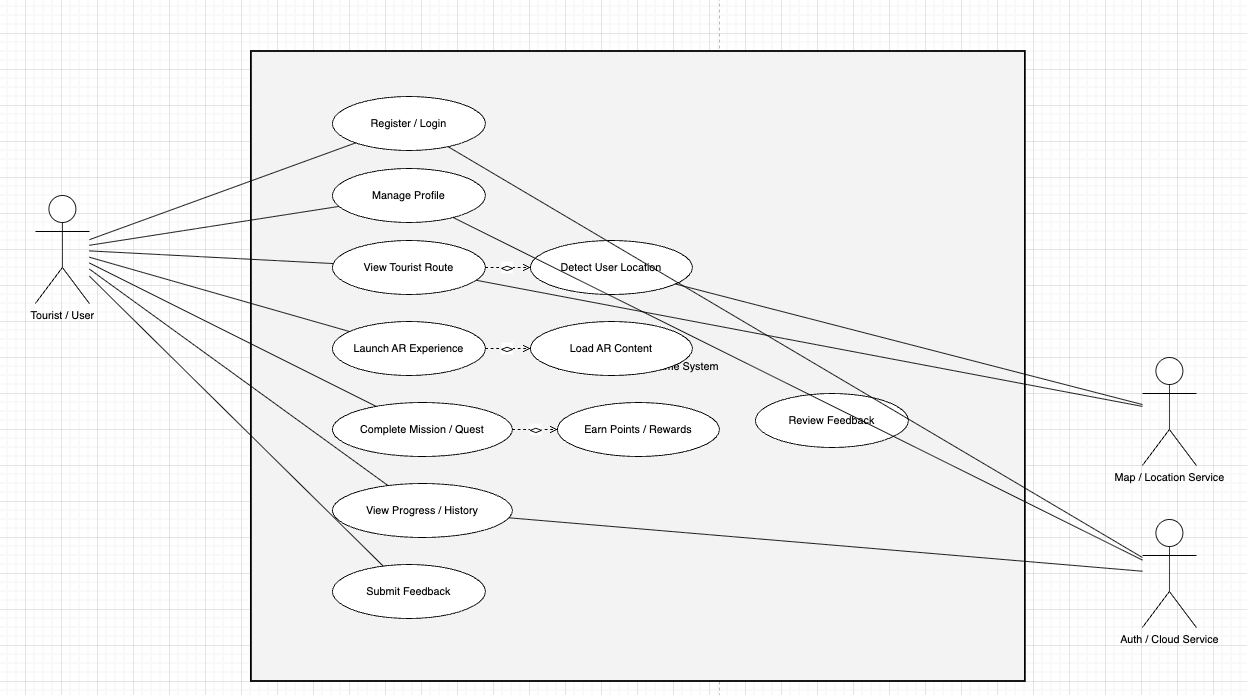
\includegraphics[width=0.8\textwidth]{figures/userflow.png}
    \caption{Хэрэглэгч ба системийн харилцан үйлчлэлийн дараалал}
    \label{fig:sequence-diagram}
\end{figure}

Offline-first стратеги нь зөвхөн газрын зураг хадгалахыг хэлэхгүй. Map corridor, nearby POI subset, localized text/audio, critical 3D bundles, quest rules, reward tables, fallback thumbnails, emergency help screen зэрэг бүгд local cache-д байх ёстой. Mapbox-ийн албан ёсны offline баримт бичиг geographic region/bounding box, zoom range, style URL шаарддагийг тодорхой заасан. OSM-ийн албан ёсны бодлого нь өөрийн tile server дээр offline prefetch хориглодог тул OSM ашиглах бол self-host, commercial OSM provider, эсвэл vector-tile pipeline төлөвлөх ёстой.

%----------------------------------------------------------------------
\section*{Контент хүргэлт, серверийн архитектур ба CMS}
%----------------------------------------------------------------------

Мобайл AR аяллын тоглоомын контентыг metadata ба binary asset гэсэн хоёр өөр ангиар удирдах нь оновчтой. Metadata нь POI, quest, trigger rule, eligibility, locale, content schedule, moderation state, reward logic, analytics taxonomy зэрэг богино JSON/Proto төрлийн өгөгдөл байна. Binary asset нь image, audio, video, subtitle, GLB/glTF, texture, lightmap, terrain patch, map pack зэрэг том объект байна. Энэ салгалтгүй бол cache policy, invalidation, localization, entitlement, bandwidth control бүгд хутгалддаг.

\begin{table}[H]
\centering
\caption{CDN сонголтын харьцуулалт}
\label{tab:cdn-comparison}
\small
\begin{tabular}{|p{2.5cm}|p{3cm}|p{3.5cm}|p{3.5cm}|}
\hline
\textbf{Сонголт} & \textbf{Ямар төрлийн ачаалалд сайн} & \textbf{Кэшийн үндсэн логик} & \textbf{AR tourism game-д хэрэглэх байрлал} \\ \hline
AWS CloudFront & Static + dynamic web content & Edge location-оор хамгийн бага latency-тэй цэгээс түгээдэг & audio/model bundle delivery, global default CDN \\ \hline
Cloudflare CDN / Images & Static asset, image pipeline & Default CDN нь file extension-оор cache хийдэг; HTML/JSON default-аар cache хийхгүй. Images нь upload, resize, optimize, signed URL дэмждэг & User-generated photo, gallery, responsive thumbnails, premium image access control \\ \hline
Cloud CDN & HTTP(S) load-balanced content & Edge POP дээр content-ийг хэрэглэгчид ойрхон cache хийнэ & API-д ойр web asset, mixed static + short-TTL metadata \\ \hline
Media CDN & Streaming media & MIME type дээр суурилсан static caching; video/audio/image сайн, HTML/JSON default-аар cache хийхгүй & Streaming audio guide, cutscene video, media-heavy tours \\ \hline
\end{tabular}
\end{table}

Эндээс гарах гол архитектурын дүрэм энгийн: том медиа-г CDN-д, хувь хэрэглэгчээс хамаарах state-ийг origin/API-д, personalized JSON-ийг богино TTL-тэй edge cache-д байрлуул. HTML/JSON-г олон CDN default-аар static media шиг авч үздэггүй тул personalized response ба static binary asset-аа нэг гарал үүсэл, нэг cache policy, нэг URL shape дээр хутгах нь буруу.

Localized агуулгын хувьд tolгойгүй CMS (headless CMS) нь presentation-ийг backend-аас салгаж, app, web preview, kiosk, operator tool-аас нэг ижил контентын эх үүсвэр ашиглах боломж олгодог. Contentful-ийн албан ёсны баримт бичиг locale, fallback locale, wildcard locale retrieval, missing translation handling-ийг тодорхой тайлбарладаг. Strapi ч ISO code-той locale, default locale, олон хэлний content management-ийг дэмждэг. Иймд ``Quest.name\_en'', ``Quest.name\_ja'' гэх хатуу schema-гаас илүү locale-variant + fallback загвар архитектурын хувьд илүү тогтвортой.

API дизайнд resource-oriented baseline хэрэгтэй. Google Cloud-ийн API design guide нь resource-oriented design-ийг суурь чиглэл болгосон; AWS-ийн serverless microservices whitepaper нь serverless-ийг operational complexity бууруулах нэг зам гэж үздэг. Mobile AR tourism game-д content-read API, state-write API, telemetry ingest, moderation/admin API гэсэн тусдаа surface-уудтай байх нь зохистой гэсэн дүгнэлт гарна. Read-heavy localized content API-г CDN-friendly байлгаж, write-heavy progression/state API-г stronger auth/idempotency-тэй байлгах ёстой.

\begin{table}[H]
\centering
\caption{Backend архитектурын харьцуулалт}
\label{tab:backend-arch}
\small
\begin{tabular}{|p{3cm}|p{4cm}|p{3.5cm}|p{3.5cm}|}
\hline
\textbf{Архитектур} & \textbf{Хэзээ тохирох} & \textbf{Давуу тал} & \textbf{Сул тал} \\ \hline
Modular monolith & Бага/дунд баг, нэг хот эсвэл хэдхэн destination, контент iteration хурдан хийх үе & Operational simplicity, transaction boundary ойлгомжтой & Дараа нь scale domain-ыг салгах шаардлага гарч магадгүй \\ \hline
Microservices & Их хэмжээний destination, тусдаа багууд, content/state/realtime domains нь бие даан хөгжих үед & Domain isolation, deployment independence & Observability, tracing, testing, ops complexity өндөр \\ \hline
Serverless / event-driven & Burst traffic, push-triggered workflow, media processing, moderation hook, localization pipeline & Idle cost бага, event fan-out сайн, ops харьцангуй хөнгөн & Cold-start, debugging, distributed state reasoning хүндрэлтэй \\ \hline
Hybrid & Ихэнх бодит AR tourism game-д хамгийн бодитой & Core API/state нь тогтвортой service дээр, async/content workflow нь event-driven байж болно & Архитектурын хил заагийг сайн тогтоохгүй бол төвөг услын давхардал үүснэ \\ \hline
\end{tabular}
\end{table}

Концепцийн data model-ийг дараах байдлаар төсөөлөхөд сайн: POI, NarrativeNode, Quest, Trigger, AssetBundle, LocaleVariant, UserProgress, VisitSession, Entitlement, TelemetryEvent. Энд локал AR session state-ийг durable account state-оос тусад нь авч үзэх хэрэгтэй. Жишээ нь хэрэглэгчийн одоогийн pose, active anchors, frame confidence нь ephemeral state; харин badge, completed quest, unlocked bundle, purchased ticket нь durable state.

%----------------------------------------------------------------------
\section*{Бодит цагийн харилцан үйлчлэл, гүйцэтгэл ба эрчим хүч}
%----------------------------------------------------------------------

Real-time шаардлагыг нэг ангиллаар ойлгож болохгүй. AR pose update, occlusion, hit-test, light estimation зэрэг нь миллисекунд түвшний on-device local loop. Харин shared quest state, territory capture, leaderboard, team puzzle solve зэрэг нь network-mediated consistency loop. Audio/video co-op бол өөр төрлийн peer real-time. Push notification, background wake, comeback prompt зэрэг нь deferred interaction loop. Сайн архитектур эдгээрийг нэг protocol, нэг state model, нэг latency expectation-д тулгахгүй.

\begin{table}[H]
\centering
\caption{Real-time channel-ийн сонголт}
\label{tab:realtime-channels}
\small
\begin{tabular}{|p{4cm}|p{3.5cm}|p{5cm}|}
\hline
\textbf{Хэрэгцээ} & \textbf{Зохимжтой суваг} & \textbf{Яагаад} \\ \hline
Pose, tracking, occlusion, local interaction & Сүлжээгүй on-device loop & Network latency-гүй, frame-by-frame тогтвортой байдал шаарддаг \\ \hline
Shared score, puzzle state, event feed & IETF WebSocket & Full-duplex, server-тэй үргэлжилсэн хоёр чиглэлт холбоо \\ \hline
Peer voice/video эсвэл ephemeral data channel & W3C WebRTC & Real-time media + generic application data, peer-to-peer боломж \\ \hline
Re-engagement, delayed event, background refresh & Push notifications / APNs / FCM & App foreground биш үед wake/update хийхэд тохиромжтой \\ \hline
\end{tabular}
\end{table}

2024 оны open-space multiplayer AR судалгаа synchronized interaction-ийг player-to-player, multiplayer-to-one-virtual-element, multiplayer-to-physical-space гэсэн гурван үндсэн хэв маягаар ангилсан. Энэ ангилал системийн дизайн дээр их хэрэгтэй. Учир нь ``бүх хэрэглэгчид яг ижил frame харах ёстой'' гэж үзэх нь ихэнх аяллын тоглоомд буруу. Ихэнх тохиолдолд server-authoritative shared intent/state хангалттай; visual manifestation нь client бүр дээр local AR frame-д хөрвөнө. Өөрөөр хэлбэл sync хийх зүйл нь камерын кадр биш, харин semantic state байна.

Гүйцэтгэл ба батарейн талд location stack хамгийн амархан алдаа гаргадаг. Android-ын албан ёсны зөвлөмж passive location update ашиглах, timeout тавих, location updates-аа хэрэггүй болмогц устгах, geofence expiration тохируулах, background location-ийг бүү хэт ашигла гэж заадаг. Android 8.0-аас хойш background location-ийн давтамж системийн түвшинд хэдхэн удаа/цаг хэмжээнд хязгаарлагддаг тул ``app background-д ч seconds-level route correction өгнө'' гэсэн архитектур бодит биш. Аяллын тоглоомд foreground moment л high-accuracy loop ажиллаж, background үед geofence/push/event-driven model руу буух ёстой.

AR runtime талд ARCore-ийн албан ёсны performance guidance нь production build дээр thermal API ашиглан device thermals-аа ажиглах, CPU starvation үүсгэхгүй байх, ``VIO frequency low'' төрлийн дохио шалгахыг зөвлөсөн. Android 12+ үед accelerometer, gyroscope, geomagnetic sensor зэргийн sampling rate 200 Hz хүртэл, SensorDirectChannel ашиглавал ихэвчлэн 50 Hz орчимд хязгаарлагддаг. Мөн accelerometer нь бусад motion sensor-оос ойролцоогоор 10 дахин бага эрчим хүч хэрэглэдэг гэж Android баримт бичиг дурдсан. Иймд custom fusion-ийг ``хамгийн хурдан sampling = хамгийн сайн'' гэж үзэх биш, tracking confidence ба power budget-ийн тэнцвэрээр удирдах ёстой.

iOS талд ч адилхан: Apple-ийн энергийн гарын авлага unnecessary wakeup, background activity, CPU-heavy workload-оос зайлсхийхийг онцолдог. LiDAR-тай төхөөрөмжид Instant AR, depth зэрэг нь илүү хурдан, тогтвортой байж болох ч энэ нь бүх төхөөрөмжид ижил биш. Тиймд feature gating, rendering budget, thermal downgrade mode, network downgrade mode, map-only fallback mode зэрэг runtime policy заавал хэрэгтэй.

Edge offloading нь заавал хэрэгтэй бүрэлдэхүүн биш, харин selective acceleration strategy гэж үзэх нь зөв. 2025--2026 оны судалгаанууд mobile AR offloading нь latency, energy efficiency, user experience-д эерэг нөлөө үзүүлж болох ч availability, redundancy, network reliability, edge dependency гэдэг шинэ төвөг нэмдгийг харуулсан. Иймд semantic scene understanding, heavy CV inference, batch personalization, LLM-based narration compose зэрэгт edge ашиглаж болох ч core gameplay registration loop-ийг дор хаяж fallback on-device path-тай байлгах ёстой.

%----------------------------------------------------------------------
\section*{Нууцлал, аюулгүй байдал ба зөвшөөрөл}
%----------------------------------------------------------------------

Location, camera, microphone нь платформын түвшинд мэдрэмтгий мэдээлэл гэж үзэгддэг. Android-ын privacy guidance нь эдгээр permission-үүд хэрэглэгчийн хувийн мэдээлэлд онцгой нөлөөтэйг тодорхой хэлдэг. iOS/macOS талд хэрэглэгч app бүрт camera, microphone permission-ээ шууд өгдөг ба camera usage indicator, microphone indicator зэрэг ил тод байдлын механизм үйлчилдэг. Иймд AR tourism game permission request-ээ onboarding дээр бөөнөөр нь авах бус, хэрэгцээ гарсан мөчид progressive байдлаар тайлбарлаж авах нь зүйтэй.

Байршлын хувьд minimum necessary scope бол үндсэн дүрэм. Android location permission docs foreground/background, fine/coarse ялгааг тодорхой заадаг; Apple-ийн Core Location docs ``When In Use'' ба ``Always'' authorization-ийг ялгадаг; iOS reduced accuracy болон temporary full accuracy request хийж болдог; Google Play-ийн бодлого minimum scope буюу coarse over fine, foreground over background хандлагыг санал болгодог. Иймд default стратеги нь foreground + approximate/reduced accuracy, харин зөвхөн бодит тоглоомын мөчид temporary precise upgrade хүсэх хэлбэр байвал хэрэглэгчийн итгэл, store compliance, батарейн хэрэглээ гурвыг зэрэг хамгаална.

Аюулгүй байдлын түвшинд хамгийн чухал нь server authority ба content boundary юм. Reward, inventory, badge, quest completion, paid entitlement, anti-cheat-sensitive state-ийг client authoritative байлгаж болохгүй. Харин static media, public POI metadata, generic route graph зэрэг нь CDN-friendly public content байж болно. Cloudflare Images нь signed URL дэмждэг; Cloud CDN ч signed URL/invalidations зэрэг secure delivery mechanism-ийг санал болгодог. Иймд ``public static'' ба ``private/per-user'' контентын хилийг архитектурын эхэнд тогтоовол privacy, caching, access control, piracy control зэрэг асуудал хөнгөрнө.

Нууцлалын өөр нэг чухал зарчим бол raw data-г удаан хадгалахгүйгээр semantic event рүү буулгах явдал юм. Жишээлбэл ``raw GPS trail'' хадгалах шаардлагагүй бол ``entered geofence X'', ``completed POI Y near 14:10'', ``played audio guide Z in locale mn-MN'' гэх event-үүдээр орлуулж болно. Мөн iOS дээр background-д camera access disabled байдаг тул foreground AR boundary-г архитектурын хатуу хязгаар гэж үзэх нь зөв.

%----------------------------------------------------------------------
\section*{Талбайн QA ба баталгаажуулалт}
%----------------------------------------------------------------------

Field condition-т ажиллах AR тоглоомын QA нь зөвхөн unit test, emulator test-ээр дуусахгүй. Үүнийг дор хаяж capability QA, spatial QA, permission QA, network QA, thermal QA, narrative QA гэсэн давхаргад хуваах хэрэгтэй. Platform behavior өөрөө олон хувьсагчтай: approximate location, reduced accuracy, missing sensor, degraded heading, no network, bad light, glare, crowd occlusion, urban canyon, indoor/outdoor threshold, battery saver, thermal throttling гэх мэт.

Android location testing guidance нь approximate location permission-тэй үед use case ажилласаар байх ёстойг тодорхой хэлдэг. Apple Xcode test plan-аар simulated location өгч болдог. Android emulator нь accelerometer, magnetometer, light зэрэг virtual sensor control-уудтай. Иймд QA matrix-д дор хаяж дараах тэнхлэгүүд орно: permission mode, device class, sensor availability, connectivity profile, route type, lighting condition, localization completeness. ``GPS зөв ажиллаж байна уу?'' гэдэг дан шалгалт хангалтгүй; ``approximate location үед core loop survive хийж байна уу?'' гэдэг нь илүү чухал.

ARCore-ийн Recording \& Playback API нь camera video stream, IMU data, custom metadata-г MP4-д хадгалж, дараа нь live session мэт playback хийх боломжтой. Энэ нь field bug-ийг deterministic regression test болгох маш хүчтэй арга юм. Жишээлбэл нэг тодорхой гудамжинд нарны хурц тусгалтай үед tracking алдагдсан бол QA баг тэр session-ийг дахин давтаж reproduce хийж чадна. ARCore performance guidance мөн production build дээр thermal API ашиглан benchmark хийхийг зөвлөдөг. Товчхондоо, ``record once, replay many'' стратеги бол outdoor AR QA-ийн гол арга юм.

Талбайн acceptance критерийг зөвхөн crash-free rate-ээр хэмжиж болохгүй. Spatial KPI-д tracking loss frequency, anchor drift incident, geofence false-positive/false-negative, route deviation recovery time, asset cache hit rate, battery drain per session, thermal-throttle incidence, locale fallback rate, notification delivery success, offline resume success зэрэг үзүүлэлтүүд орно. Судалгааны хувьд HeritageSite AR зэрэг 2024 оны ажил immersive storytelling ба heritage experience-ийг mobile AR exploration game-аар баяжуулж болдгийг харуулж байгаа бол 2024 оны аялал жуулчлалын field experiment хэт удирдсан маршрутын сөрөг нөлөөг сануулж байна. Иймд QA нь зөвхөн техникийн тогтвортой байдал биш, мөн орчны эрх чөлөө ба narrative flexibility-г баталгаажуулах ёстой.

Эцсийн дүгнэлт нь энгийн боловч системийн хувьд ачаалалтай: сайн мобайл AR tourism game нь AR registration-ээ локалд, географ логикоогоо бүсийн түвшинд, контент хүргэлтээ cache-friendly хэлбэрээр, state-ээ authoritative backend-д, permission ба QA-гаа эхнээс нь төлөвлөсөн байх ёстой. Энэ таван зарчмыг баримталбал платформ, вендор, SDK, map provider, realtime layer, localization stack өөрчлөгдсөн ч системийн суурь нь тогтвортой үлдэнэ.

\end{sloppy}